\documentclass{fict}
\addbibresource{references.bib}

\newglossaryentry{xhat}{
    name=\ensuremath{\hat{x}(n)},
    description={Estimated enhanced speech signal at sample \(n\)},
    sort=hatx,
    type=main
}
\newglossaryentry{xhatomega}{
    name=\ensuremath{\hat{x}(\omega)},
    description={Estimated enhanced speech signal in the frequency domain},
    sort=hatxomega,
    type=main
}
\newglossaryentry{x}{
    name=\ensuremath{x(n)},
    description={Clean reference speech signal at sample \(n\)},
    sort=x,
    type=main
}
\newglossaryentry{N}{
    name=\ensuremath{N},
    description={Total number of samples in the signal},
    sort=N,
    type=main
}
\newglossaryentry{Ps}{
    name=\ensuremath{P_s},
    description={Power of the clean speech signal},
    sort=Ps,
    type=main
}
\newglossaryentry{Pn}{
    name=\ensuremath{P_n},
    description={Power of the noise (or error) signal},
    sort=Pn,
    type=main
}
\newglossaryentry{Sft}{
    name=\ensuremath{S(f, t)},
    description={Clean magnitude spectrum at frequency bin \(f\), time frame \(t\)},
    sort=S,
    type=main
}
\newglossaryentry{Shft}{
    name=\ensuremath{\hat{S}(f, t)},
    description={Enhanced magnitude spectrum at frequency bin \(f\), time frame \(t\)},
    sort=Sh,
    type=main
}
\newglossaryentry{Xomega}{
    name=\ensuremath{|X(\omega)|},
    description={Magnitude spectrum of the clean signal},
    sort=X,
    type=main
}
\newglossaryentry{Yomega}{
    name=\ensuremath{|Y(\omega)|},
    description={Magnitude spectrum of the noisy speech},
    sort=Y,
    type=main
}
\newglossaryentry{Domega}{
    name=\ensuremath{|D(\omega)|},
    description={Estimated magnitude spectrum of the noise},
    sort=D,
    type=main
}
\newglossaryentry{Homega}{
    name=\ensuremath{H(\omega)},
    description={Frequency-dependent Wiener gain},
    sort=H,
    type=main
}
\newglossaryentry{xi}{
    name=\ensuremath{\xi},
    description={A priori signal-to-noise ratio (SNR)},
    sort=xi,
    type=main
}
\newglossaryentry{gamma}{
    name=\ensuremath{\gamma},
    description={A posteriori signal-to-noise ratio (SNR)},
    sort=gamma,
    type=main
}
\newglossaryentry{nu}{
    name=\ensuremath{\nu},
    description={Intermediate variable in MMSE-LSA used in gain estimation},
    sort=nu,
    type=main
}

% Acronyms

\newacronym[description=Machine Learning]{ml}{ML}{Machine Learning}
\newacronym[description=Artificial Intelligence]{ai}{AI}{Artificial Intelligence}
\newacronym[description=Digital Signal Processing]{dsp}{DSP}{Digital Signal Processing}
\newacronym[description= Active Noise Cancellation]{anc}{ANC}{Active Noise Cancellation}
\newacronym[description=Out-Of-Memory]{oom}{OOM}{Out-Of-Memory}

\newacronym[description=Spectral Subtraction]{ss}{SS}{Spectral Subtraction}
\newacronym[description=Wiener Filtering]{wf}{WF}{Wiener Filtering}
\newacronym[description=Minimum Mean-Square Error Log-Spectral Amplitude]{mmse-lsa}{MMSE-LSA}{Minimum Mean-Square Error Log-Spectral Amplitude}

\newacronym[description=Short-Time Fourier Transform]{stft}{STFT}{Short-Time Fourier Transform}
\newacronym[description=Fast Fourier Transform]{fft}{FFT}{Fast Fourier Transform}
\newacronym[description=Inverse Short-Time Fourier Transform]{istft}{ISTFT}{Inverse Short-Time Fourier Transform}

\newacronym[description=Signal-to-Noise Ratio]{snr}{SNR}{Signal-to-Noise Ratio}
\newacronym[description=Mean Squared Error]{mse}{MSE}{Mean Squared Error}
\newacronym[description=Perceptual Evaluation of Speech Quality]{pesq}{PESQ}{Perceptual Evaluation of Speech Quality}
\newacronym[description=Short-Time Objective Intelligibility]{stoi}{STOI}{Short-Time Objective Intelligibility}
\newacronym[description=Log-Spectral Distance]{lsd}{LSD}{Log-Spectral Distance}
\newacronym[description=Equal Error Rate]{eer}{EER}{Equal Error Rate}

\newacronym[description=Fully Convolutional Network]{fcn}{FCN}{Fully Convolutional Network}

\newacronym[description=Padding-Truncation Output-Truncation]{pto}{PTO}{Padding-Truncation Output-Truncation}
\newacronym[description=Convolutional Neural Network]{cnn}{CNN}{Convolutional Neural Network}
\newacronym[description=Convolutional Encoder-Decoder]{ced}{CED}{Convolutional Encoder-Decoder}
\newacronym[description=Residual Convolutional Encoder-Decoder]{rced}{R-CED}{Residual Convolutional Encoder-Decoder}
\newacronym[description=U-shaped Convolutional Neural Network]{unet}{UNet}{U-shaped Convolutional Neural Network}
\newacronym[description=Convolutional Time-domain Audio Separation Network]{convtasnet}{Conv-TasNet}{Convolutional Time-domain Audio Separation Network}
\newacronym[description=Temporal Convolutional Network]{tcn}{TCN}{Temporal Convolutional Network}

\newacronym[description=Group Normalization]{gn}{GN}{Group Normalization}
\newacronym[description=Batch Normalization]{bn}{BN}{Batch Normalization}
\newacronym[description=Rectified Linear Unit]{relu}{ReLU}{Rectified Linear Unit}
\newacronym[description=Parametric Rectified Linear Unit]{prelu}{PReLU}{Parametric Rectified Linear Unit}
\newacronym[description=Garbage Collection]{gc}{GC}{Garbage Collection}
\newacronym[description=16-bit Floating Point]{fp16}{FP16}{16-bit Floating Point}
\newacronym[description=32-bit Floating Point]{fp32}{FP32}{32-bit Floating Point}


\newacronym[description=Visual Studio Code]{vscode}{VSCode}{Visual Studio Code}
\newacronym[description=Secure Shell]{ssh}{SSH}{Secure Shell}


\title{Machine Learning Noise Cancellation \\ System}
\author{Graham Pellegrini}
\supervisor{Dr Ing. Trevor Spiteri}
\degreename{Bachelor of Science (Honours) (Computer Engineering)}
\titledate{June 2025}

\begin{document}

\frontmatter{}
\pagestyle{pageNumbersOnly}

\makeatletter
\begin{titlepage}
    \begin{flushleft}
        \begin{minipage}[t][5.2cm][t]{\textwidth}
            \begin{Huge}
                \textbf{\@title}
            \end{Huge}
        \end{minipage}
        %
        \begin{minipage}[t][1.3cm][t]{\textwidth}
            \begin{LARGE}
                \textbf{\@author}
            \end{LARGE}
        \end{minipage}
        %
        \begin{minipage}[t][3.9cm][t]{\textwidth}
            \begin{Large}
                \begin{tabular}{@{}ll@{}}
                    Supervisor:    & \@supervisor{}   \\
                    \ifdefined\@cosupervisor{}%
                    Co-Supervisor: & \@cosupervisor{} \\
                    \fi%
                \end{tabular}
            \end{Large}
        \end{minipage}
        %
        \begin{minipage}[t][9.5cm][t]{\textwidth}
            \begin{Large}
                \@titledate{}
            \end{Large}
        \end{minipage}
        %
        \begin{large}
            \textit{Submitted in partial fulfilment of the requirements}
            \newline
            \textit{for the degree of \@degreename{}.}
        \end{large}

        \vfill

        
\includegraphics[width=9.4cm,keepaspectratio]{content/figures/ict_logo}
    \end{flushleft}
\end{titlepage}
\makeatother

\chapter*{Abstract}
\addcontentsline{toc}{chapter}{Abstract}

Lorem ipsum dolor sit amet, consectetur adipiscing elit.
Mauris sed ipsum risus.
Nulla aliquet quis quam sed eleifend.
Donec rutrum, dolor id vulputate pharetra, nulla tortor laoreet nisl,
pellentesque dapibus velit dolor suscipit purus.
Phasellus vitae eleifend sem.
Integer ultricies ex in neque pellentesque, vitae facilisis orci aliquam.
In pellentesque mollis turpis, eu tristique lacus eleifend nec.
Vestibulum orci neque, rhoncus vitae convallis eu, suscipit quis dui.
Nulla libero elit, porta sit amet sagittis vel, placerat sit amet tortor.
Aliquam hendrerit dolor sit amet sollicitudin ornare.
Aliquam placerat sodales est, in vestibulum nisl efficitur in.
Nulla venenatis aliquam sem, at volutpat nisl pellentesque eleifend.
Praesent vitae euismod nulla, eget vehicula turpis.
Duis quis tellus vitae nisi tempus tincidunt.

Nam quis aliquet nisi, non pharetra ligula.
Phasellus pulvinar mattis neque, nec interdum justo condimentum hendrerit.
Mauris fermentum venenatis faucibus.
Pellentesque egestas eleifend libero, quis placerat ante fermentum et.
Suspendisse accumsan gravida rhoncus.
Vestibulum auctor sodales vehicula.
Pellentesque a urna et elit placerat laoreet a quis turpis.
Morbi ut sem at nunc posuere malesuada vel nec libero.
Nam et urna suscipit, bibendum diam sed, aliquet leo.
Lorem ipsum dolor sit amet, consectetur adipiscing elit.
Ut pretium mauris et nulla malesuada, mattis tristique lectus molestie.
Aenean accumsan iaculis quam, eget varius libero placerat eu.
Fusce mauris justo, vulputate a sollicitudin a, malesuada at est.
Sed ac augue elit.
Maecenas massa lorem, tincidunt vitae neque et, maximus dictum tellus.

\chapter*{Acknowledgements}
\addcontentsline{toc}{chapter}{Acknowledgements}

I would first like to express my sincere gratitude to the Faculty of ICT for their continuous support throughout my undergraduate studies. As a student athlete, I faced the dual responsibility of fulfilling both national athletic commitments and academic requirements. The department’s understanding and cooperation were invaluable in helping me persue both responsibilities.

A special thanks to my supervisor Dr Ing. Trevor Spiteri for his guidance and support during this project. His expertise and insights were instrumental in shaping the direction of my research. 

I would also like to thank my parents for their unwavering support in all my endeavours. Their belief in my decisions and the stability they provide is essential in allowing me to fully commit to my academic journey. Lastly, a heartfelt thank you to my sister, who will soon make me an uncle.
\clearpage{}

\tableofcontents{}
\addcontentsline{toc}{chapter}{Contents}
\clearpage{}

\listoffigures{}
\addcontentsline{toc}{chapter}{List of Figures}
\clearpage{}

\listoftables{}
\addcontentsline{toc}{chapter}{List of Tables}
\clearpage{}

\printglossary[type=\acronymtype,nonumberlist,title=List of Abbreviations]
\addcontentsline{toc}{chapter}{List of Abbreviations}
\clearpage{}

\printglossary[nonumberlist,title=Glossary of Symbols]
\addcontentsline{toc}{chapter}{Glossary of Symbols}
\clearpage{}

\mainmatter{}
\pagestyle{MainMatter}

\graphicspath{{content/chapters/1_introduction/figures}}
\chapter{Introduction}
\label{chp:introduction}

Machine learning, commonly referred to as Artificial Intelligence (AI), has seen rapid advancements over the past decade. These advancements have been largely driven by increasing computational power and the availability of large datasets. As a result, machine learning techniques have been integrated into various domains to solve complex problems, including speech processing and noise cancellation. However, this shift toward AI-driven solutions has often lacked thorough evaluation, with justifications for their use and the required computational resources sometimes being unclear.

This project focuses on noise cancellation in audio signals for speech enhancement, a critical area with applications in telecommunications, assistive technologies, and real-time communication systems. Noise is defined as the attenuation or distortion of an original signal caused by external factors, including background sounds in an environment or interference from electronic devices. Background noise can significantly degrade the quality of speech signals, making it difficult to understand or process the conveyed information. Noise can be classified into two categories: stationary and non-stationary \cite{loizou2013speech}.

\begin{itemize}
    \item Stationary noise has a constant power spectral density, meaning its properties remain relatively unchanged over time. An example is white noise, which is random but statistically stable.
    \item Non-stationary noise has a varying power spectral density, meaning its characteristics fluctuate over time. Examples include traffic noise or human chatter, which are unpredictable and more difficult to remove.
\end{itemize}

Two fundamental characteristics of speech are utilized in speech enhancement. Firstly, speech is a non-stationary signal, which helps in distinguishing it from stationary noise. Secondly, speech has a specific frequency range, typically between 300 Hz and 3400 Hz, known as the human voice frequency range. This allows filtering techniques to remove non-speech components while preserving intelligibility.

Noise cancellation is the process of removing unwanted noise from a signal, allowing the original speech to be heard more clearly. Traditional noise cancellation techniques, such as the Wiener filter, estimate and subtract noise from the signal. However, these classical methods often assume stationary noise, which is not always the case in real-world environments. Machine learning-based approaches have emerged as a promising alternative, offering the ability to learn complex patterns and relationships in data without requiring explicit rule-based programming.

\section{Neural Networks for Noise Cancellation}
\label{sec:neural_networks}

Machine learning models, particularly neural networks, have been widely adopted for noise cancellation. Neural networks, inspired by biological neurons in the human brain, are composed of layers of interconnected processing units known as \textit{neurons}. Each artificial neuron receives multiple inputs, performs a weighted summation, applies a bias, and passes the result through an activation function to produce its output.

This structure draws direct inspiration from the way biological neurons function—where dendrites receive signals, the cell body processes them, and the axon transmits the signal to the next neuron. Figure~\ref{fig:neuron_vs_ann} illustrates this analogy.

\begin{figure}[H]
    \centering
    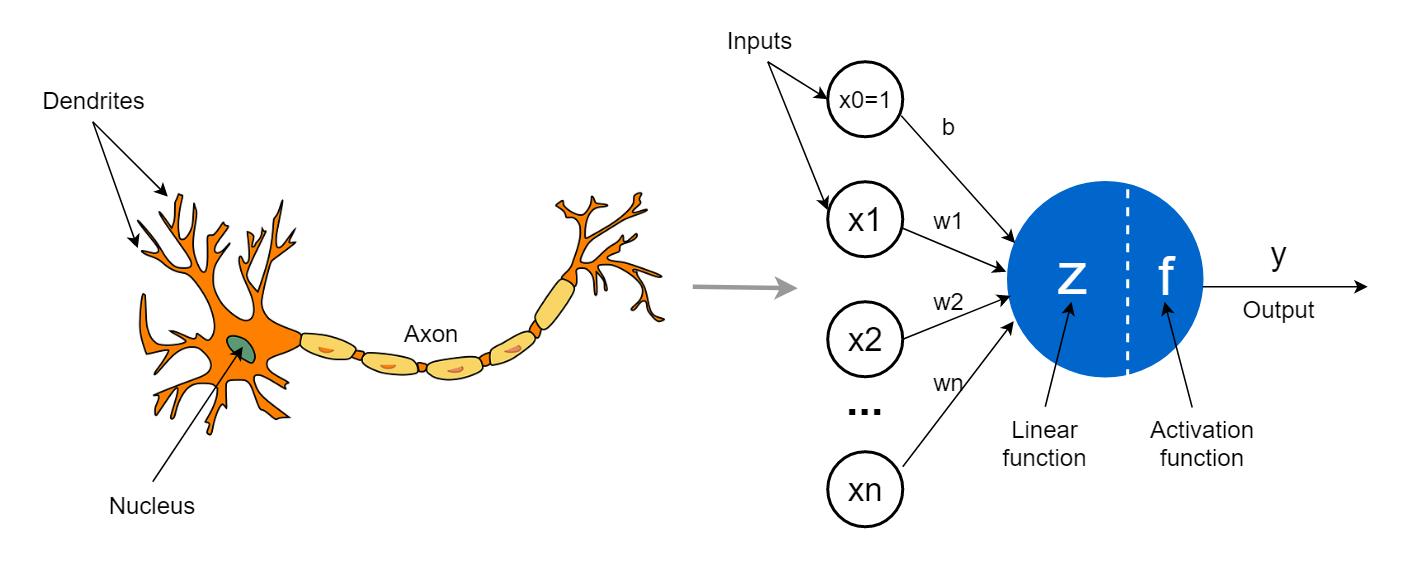
\includegraphics[width=0.75\textwidth]{neuron_vs_ann.png}
    \caption{Biological neuron vs. Artificial neuron structure.\cite{ghosh2020perceptron}}
    \label{fig:neuron_vs_ann}
\end{figure}

A typical neural network for noise cancellation consists of the following components:
\begin{itemize}
    \item \textbf{Input layer:} Receives the noisy speech signal (e.g., a time-domain waveform or its spectrogram).
    \item \textbf{Hidden layers:} Perform nonlinear transformations to extract key features and patterns from the input. These layers may include convolutional, recurrent, or fully connected neurons depending on the network architecture.
    \item \textbf{Output layer:} Produces the denoised speech signal by mapping the learned features back to the clean signal domain.
\end{itemize}

The network is trained using pairs of clean and noisy audio samples. It gradually learns to reduce the difference between its predicted output and the actual clean signal. Once trained, the model can take in new noisy speech and output a cleaner version. This learning-based approach allows neural networks to adapt to complex noise patterns, often performing better than traditional signal processing methods in real-world situations.

\section{Project Goals and Implementation}

The primary goal of the project is to explore both classical and machine learning-based approaches to noise cancellation, evaluating their effectiveness and feasibility in real-world applications. The project will not only examine established noise reduction techniques but also develop a machine learning-based model, comparing its performance against classical methods.

The approach involves designing and implementing a noise cancellation system that operates under the assumption of a single-speaker scenario in a noisy background environment, where the system must remove both stationary and non-stationary noise without access to a clean reference signal. Unlike established pre-trained models that required extensive datasets and resources, the model developed in this project will not be pre-trained, allowing for a demonstration of the ease of developing and training in practical settings. However, during evaluation and benchmarking, pre-trained models will be used for comparison to assess their effectiveness against the proposed approach.

The project will be implemented in Python using a modular and reproducible structure, ensuring that the framework can be extended or modified for further improvements. The project is structured into three core phases: training, denoising, and deployment
\begin{itemize}
    \item Training phase: The most computationally intensive stage, where a sourced dataset of clean and noisy speech samples will be formatted and fed into the model to learn respective mapping.
    \item Denoising phase: Involves loading the trained model and applying it to a noisy speech signal to generate a cleaned output. Here evalution metrics will also be producable to assess the performance of one methodology against another.
    \item Deployment phase: The final phase involves simulating a real-world application scenario. After training ad justification through performance evaluation, the model will be embedded into a real-time application. This will essentially be a remake of the denoising phase, but with the model integrated into a board that will take real time input sequence from a microphone and save the denoised output. The label for real-time will be indicated through evaluated inference time calculated during the denoising phase.
\end{itemize}


\section{Overview of the Contents of the Report}
\graphicspath{{content/chapters/2_background/figures/}}
\chapter{Background}
\label{chp:background}

In this chapter, background information on established classical noise reduction methods is provided. These methods align with the scope of the project in that they do not require any reference or clean signal to base their predictions on. The chapter explores the Spectral Subtraction method and the Wiener Filtering method. Additionally, a brief section outlining the progression of the project and relevant foundational knowledge is included.

\section{Spectral Subtraction}
\label{sec:spectral_subtraction}

Spectral Subtraction is one of the most widely used techniques for single-channel speech enhancement. The core idea is to estimate the noise spectrum from a noisy speech signal and subtract it from the observed spectrum to obtain a cleaner signal \cite{loizou2013speech}. It assumes that noise remains relatively stationary over short time frames, while speech is a dynamic, non-stationary signal.

For digital signal processing to occur, the analog speech signal \(x(t)\), which is continuous in time, must first be converted into a digital signal \(x[n]\), a discrete-time representation. This digitisation must satisfy the Nyquist criterion: the sampling rate should be at least twice the maximum frequency component present in the signal to ensure accurate reconstruction. However, sampling inherently introduces limitations. Quantisation noise, resulting from the finite precision of digital systems, and aliasing, caused by inadequate sampling rates, can degrade the signal. If the sampling rate is too low, high-frequency components may fold into lower frequencies, misrepresenting the signal content.

\begin{figure}[h]
    \centering
    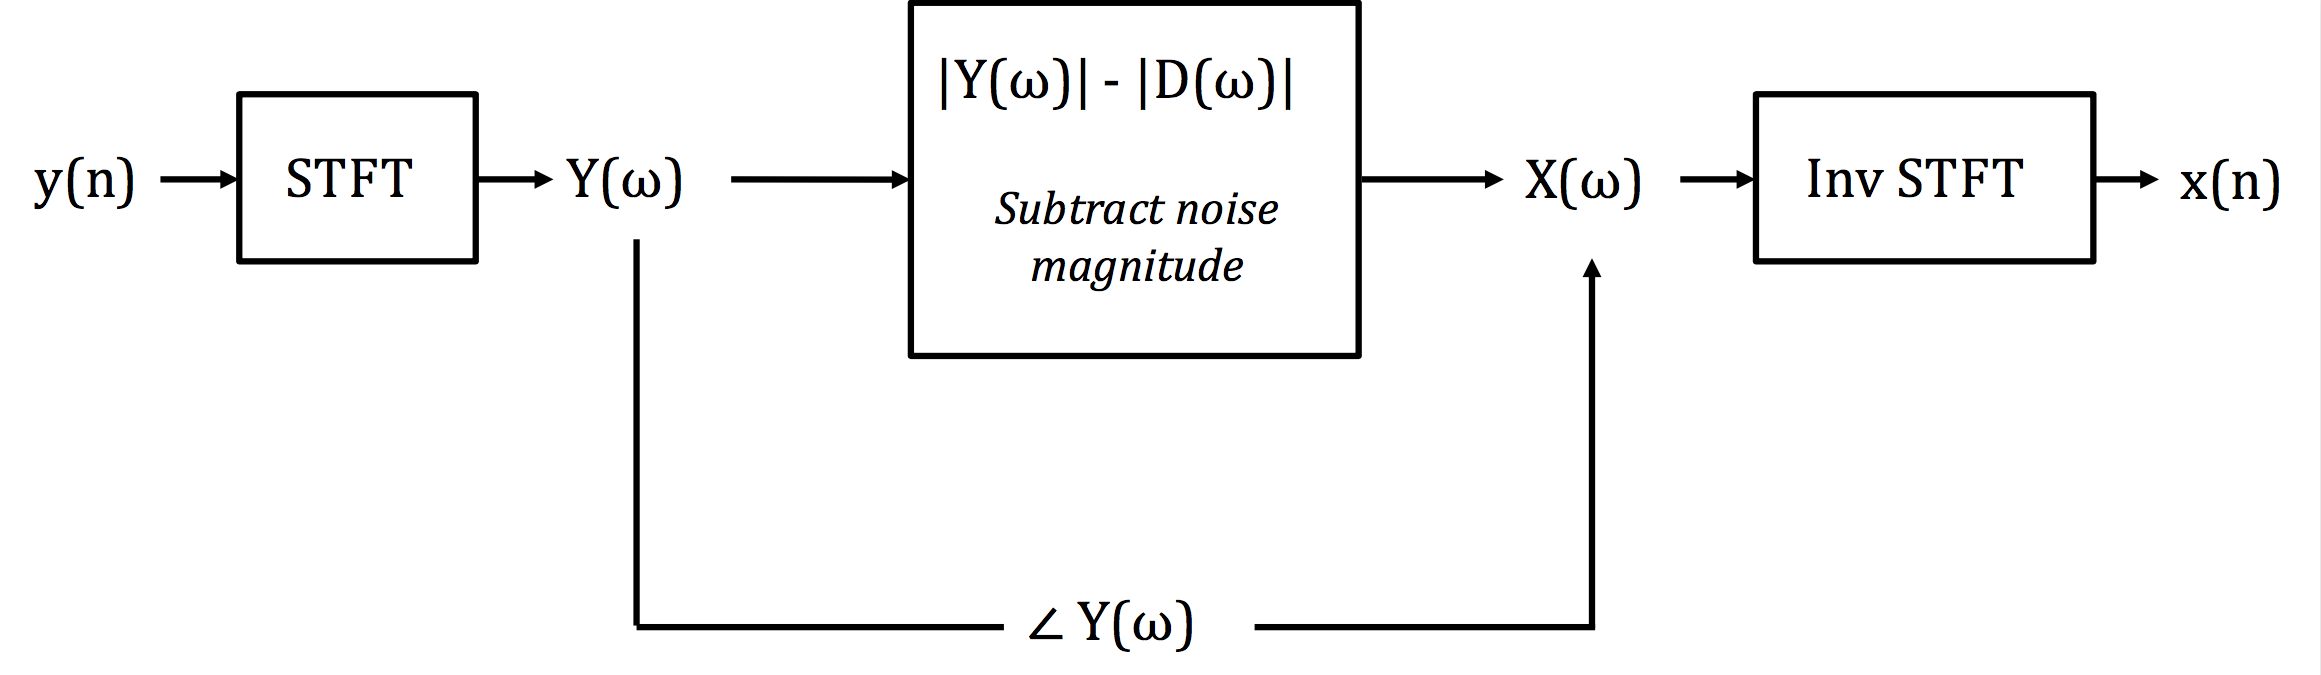
\includegraphics[width=\textwidth,keepaspectratio]{specsub.png}
    \caption{\label{fig:SSBlock} Block diagram of the Spectral Subtraction method \cite{dubey2016evaluation}.}
\end{figure}

Before applying spectral subtraction, the signal is pre-processed into a suitable format using the Short-Time Fourier Transform (STFT). The STFT segments the time-domain signal into overlapping frames using a windowing function and then converts each segment into the frequency domain. Windowing reduces spectral leakage and preserves continuity in the frequency domain. The magnitude spectrum of the noisy signal is obtained by taking the absolute value of the STFT \cite{dubey2016evaluation}. The noise spectrum is estimated by averaging the spectral magnitudes of non-speech segments over time. Once this estimate is obtained, it is subtracted from the noisy spectrum to yield an estimate of the clean speech. The final step applies the Inverse Short-Time Fourier Transform (ISTFT) to reconstruct the enhanced signal in the time domain by summing the overlapping frames.

This process can be mathematically described as:

\begin{equation}
    |X(\omega)| = |Y(\omega)| - |D(\omega)|
\end{equation}

where:
\begin{itemize}
    \item \( X(\omega) \): Estimated clean speech spectrum,
    \item \( Y(\omega) \): Magnitude spectrum of the noisy speech,
    \item \( D(\omega) \): Estimated noise spectrum.
\end{itemize}

Spectral subtraction is widely adopted due to its simplicity and low computational cost. It requires only a single input channel and is straightforward to implement. However, it comes with notable limitations. It assumes stationary noise—a condition often unmet in real environments—and may introduce **musical noise**, a type of distortion perceived as tonal artifacts. Additionally, excessive subtraction may distort speech, while insufficient subtraction can leave residual noise.

Despite these challenges, spectral subtraction remains a valuable baseline for evaluating more advanced noise suppression techniques. Methods such as Wiener filtering and deep learning-based approaches have been developed to overcome these shortcomings through more adaptive or data-driven mechanisms \cite{loizou2013speech}.


\section{Wiener Filtering}
\label{sec:wiener_filtering}

Wiener filtering is a statistically grounded method for speech enhancement that aims to minimise the mean square error (MSE) between the estimated clean signal and the true clean signal \cite{loizou2013speech}. Originally developed for linear time-invariant systems, the Wiener filter assumes that both the signal and noise are stationary stochastic processes and seeks the optimal linear estimate of the clean speech given the noisy observation \cite{dubey2016evaluation}.

The method can be applied in both the time domain and frequency domain, though the frequency domain approach is more common in speech processing due to its computational efficiency and alignment with standard short-time signal representations. The key idea is that if the power spectral densities (PSDs) of the clean speech \(P_S(\omega)\) and the noise \(P_N(\omega)\) are known or can be estimated, the optimal filter \(H(\omega)\) is derived as:

\begin{equation}
    H(\omega) = \frac{P_S(\omega)}{P_S(\omega) + P_N(\omega)}
\end{equation}

This filter acts as a frequency-dependent gain function. Frequencies where the clean speech dominates (\(P_S \gg P_N\)) are preserved, while noise-dominant frequencies (\(P_N \gg P_S\)) are attenuated. The enhanced speech spectrum is obtained by multiplying the noisy spectrum \(Y(\omega)\) with the Wiener gain:

\begin{equation}
    \hat{X}(\omega) = H(\omega)Y(\omega)
\end{equation}

Following this, the enhanced time-domain signal is reconstructed using the Inverse Short-Time Fourier Transform (ISTFT).

\begin{figure}[h]
    \centering
    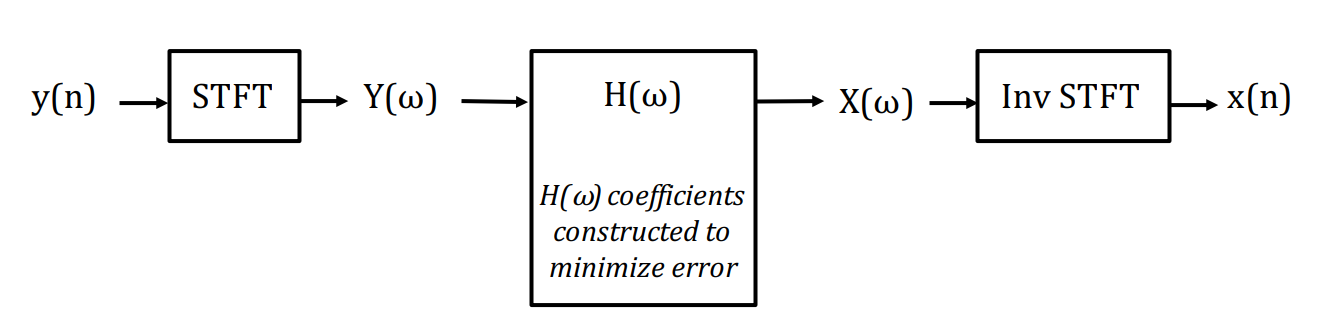
\includegraphics[width=0.95\textwidth,keepaspectratio]{wiener_block.png}
    \caption{\label{fig:WienerBlock} Block diagram of the Wiener filtering process \cite{dubey2016evaluation}.}
\end{figure}

In the time domain, the Wiener filter can be derived through a least mean square (LMS) optimisation approach. Consider a noisy signal \( y(n) = x(n) + d(n) \), where \( x(n) \) is the clean signal and \( d(n) \) is the noise. The filter \( h(n) \) is constructed to minimise the expected squared error:

\begin{equation}
    J = E\left[ (x(n) - \hat{x}(n))^2 \right]
\end{equation}

Expanding this using the LMS framework, the optimal filter is:

\begin{equation}
    h = R_{yy}^{-1} r_{yx}
\end{equation}

where \( R_{yy} \) is the autocorrelation matrix of the noisy signal and \( r_{yx} \) is the cross-correlation vector between the noisy and clean signals. The result is then convolved with \( y(n) \) to obtain the enhanced estimate \( \hat{x}(n) \).

Wiener filtering is particularly advantageous when the noise characteristics can be reliably estimated, such as during silent segments of speech. However, it assumes that the noise is zero-mean and uncorrelated with the speech signal, which may not always hold in practice. Additionally, in highly non-stationary environments, its performance can degrade due to inaccurate PSD estimates.Compared to spectral subtraction, Wiener filtering provides a more principled and statistically optimal approach, balancing noise suppression and speech preservation based on spectral power estimates. It introduces less musical noise and generally achieves better perceptual quality in stationary noise conditions.

Wiener filtering can be seen toprovide an optimal solution in the minimum mean square error (MMSE) sense. It is able to retain the spectral shape of speech components better than spectral subtraction, making it a more effective method for speech enhancement. The Wiener filter is adaptable to both time and frequency domain implementations, allowing for flexibility in its application. However, it assumses stationary noise and accurate noise estimation, which may not always hold in real-world scenarios. This can lead to over-smoothing, reducing speech intelligibility. Additionally, the performance of Wiener filtering can degrade in highly dynamic or non-stationary noise conditions.

Despite its assumptions, Wiener filtering is still widely used as a foundational method in speech enhancement and often forms part of more complex hybrid pipelines or adaptive filtering systems \cite{dubey2016evaluation, loizou2013speech}.


\section{Evaluation Metrics}
\label{sec:evaluation_metrics}

To evaluate the performance of noise reduction algorithms, several objective metrics are commonly used. These metrics provide quantitative measures of the quality and intelligibility of enhanced speech signals when compared to their clean references. The following subsections describe the most widely adopted metrics in speech enhancement research, all of which are utilised in this project.

\subsection{Signal-to-Noise Ratio (SNR)}
\label{subsec:snr}

The Signal-to-Noise Ratio (SNR) is a fundamental metric that quantifies the relative strength of the desired speech signal compared to the background noise. A higher SNR indicates better separation between speech and noise components, which typically translates to improved intelligibility and perceived quality.

SNR is defined as:

\begin{equation}
    \text{SNR} = 10 \log_{10} \left( \frac{P_s}{P_n} \right)
\end{equation}

where \( P_s \) is the power of the clean speech signal and \( P_n \) is the power of the noise (or error) component. In practice, SNR can be computed in both time and frequency domains and is commonly used as a baseline performance indicator for denoising systems.

\subsection{Mean Squared Error (MSE)}
\label{subsec:mse}

The Mean Squared Error (MSE) measures the average squared difference between the enhanced and reference clean signals. It reflects the overall fidelity of the enhancement process but does not necessarily correlate with perceptual quality.

MSE is given by:

\begin{equation}
    \text{MSE} = \frac{1}{N} \sum_{n=1}^{N} (x(n) - \hat{x}(n))^2
\end{equation}

where \( N \) is the number of signal samples, \( x(n) \) is the clean signal, and \( \hat{x}(n) \) is the enhanced signal. Lower MSE values indicate better approximation of the clean signal.

\subsection{Perceptual Evaluation of Speech Quality (PESQ)}
\label{subsec:pesq}

The Perceptual Evaluation of Speech Quality (PESQ) is an objective metric designed to estimate the perceptual quality of speech, taking into account human auditory perception. Standardised by ITU-T Recommendation P.862, PESQ is widely used in speech enhancement and telecommunication systems.

PESQ simulates the auditory perception process and compares the clean and enhanced signals using psychoacoustic models. The PESQ score ranges from -0.5 to 4.5, with higher scores indicating better perceptual quality. A score above 3.0 is generally considered acceptable for most applications.

\subsection{Short-Time Objective Intelligibility (STOI)}
\label{subsec:stoi}

The Short-Time Objective Intelligibility (STOI) metric is designed to assess the intelligibility of speech, especially in noisy or distorted conditions. It works by comparing the short-time spectral envelopes of clean and enhanced speech segments.

The STOI score lies between 0 and 1, where higher values indicate better intelligibility. Scores above 0.5 typically suggest acceptable levels of speech understanding. STOI is particularly useful when intelligibility, rather than perceptual quality alone, is of primary concern.

\subsection{Log Spectral Distance (LSD)}
\label{subsec:lsd}

The Log Spectral Distance (LSD) metric quantifies the spectral distortion introduced by a denoising algorithm. It measures the average distance between the logarithmic power spectra of the clean and enhanced signals across time and frequency.

LSD is defined as:

\begin{equation}
    \text{LSD} = \frac{1}{F} \sum_{f=1}^{F} \sqrt{ \frac{1}{T} \sum_{t=1}^{T} \left( \log S(f, t) - \log \hat{S}(f, t) \right)^2 }
\end{equation}

where \( S(f, t) \) and \( \hat{S}(f, t) \) are the clean and enhanced magnitude spectra at frequency bin \( f \) and time frame \( t \), respectively. Lower LSD values indicate better preservation of spectral characteristics and less distortion.

\vspace{1em}
Individually, these metrics suffer to provide complete meaningful evaluations of the performance of noise reduction algorithms. For example, SNR and MSE are sensitive to the absolute power levels of the signals, while PESQ and STOI focus on perceptual aspects. Therefore, a comprehensive evaluation should consider multiple metrics to capture different dimensions of performance and together a well-rounded assessment can be achieved.


\section{Project Progression}
\label{sec:project_progression}

The initial objective of this project was to enhance speech signals corrupted by noise using traditional digital signal processing (DSP) techniques. The original scope involved implementing classical noise reduction methods, such as Spectral Subtraction and Wiener Filtering, with the intention of deploying them on an MSP432 microcontroller. These techniques were selected due to their low computational complexity and suitability for resource-constrained embedded systems.

However, early experimentation and prototyping conducted in Python revealed the inherent limitations of classical DSP methods—particularly their poor performance in non-stationary noise environments and lack of adaptability to diverse real-world conditions. While methods like Spectral Subtraction offer simplicity and efficiency, they tend to introduce musical noise artifacts and degrade intelligibility under dynamic noise conditions. Similarly, Wiener Filtering, though more mathematically rigorous, still relies on assumptions about the noise characteristics that may not hold in practical use cases.

Concurrently, the rising prominence of data-driven methods in the field of speech enhancement provided a compelling alternative. Established real-time systems such as \textit{Krisp}, \textit{NVIDIA RTX Voice}, and \textit{RNNoise} have demonstrated the effectiveness of deep learning-based models for robust noise suppression. These models, trained on large-scale paired datasets of clean and noisy speech, are capable of learning complex nonlinear mappings and generalising across a wide range of noise profiles.

Given these advancements, it became increasingly evident that deep learning offered significant advantages over classical methods. Consequently, the project scope evolved from solely implementing classical techniques on a low-power embedded platform to exploring the feasibility of deploying a lightweight deep learning-based speech enhancement model on a more capable microcontroller or embedded processor.

This shift allowed the project to align with modern trends in speech processing while retaining a practical, real-time deployment focus. It also opened opportunities to evaluate the trade-offs between classical and data-driven methods—not only in terms of performance but also in memory usage, computational cost, and real-world applicability.

Thus, the revised goal of the project became twofold: to benchmark deep learning-based noise suppression models against classical DSP methods across relevant objective metrics, and to assess the practicality of deploying such models on embedded hardware for real-time speech enhancement applications. Ultimately having project title revised from \textit{DSP Based Noise Cancellation System} to \textit{Machine Learning Noise Cancellation System} to reflect the new focus on deep learning techniques.

\graphicspath{{content/chapters/3_literature/figures/}}
\chapter{Literature Review}
\label{sec:literature_review}

This chapter presents an overview of relevant machine learning methods used for speech enhancement, with particular emphasis on the autoencoder architecture. It begins by introducing the fundamental principles behind neural networks and their biological inspiration, followed by a detailed discussion of machine learning techniques applied to noise suppression. Recent architectural advancements and training strategies are covered, culminating in the evaluation metrics used throughout this project to benchmark both classical and machine learning approaches.


\section{Neural Networks}
\label{sec:neural_networks}

Machine learning models, particularly neural networks, have been widely adopted for noise cancellation. Neural networks, inspired by biological neurons in the human brain, are composed of layers of interconnected processing units known as \textit{neurons}. Each artificial neuron receives multiple inputs, performs a weighted summation, applies a bias, and passes the result through an activation function to produce its output.

This structure draws direct inspiration from the way biological neurons function—where dendrites receive signals, the cell body processes them, and the axon transmits the signal to the next neuron. Figure~\ref{fig:neuron_vs_ann} illustrates this analogy.

\begin{figure}[H]
    \centering
    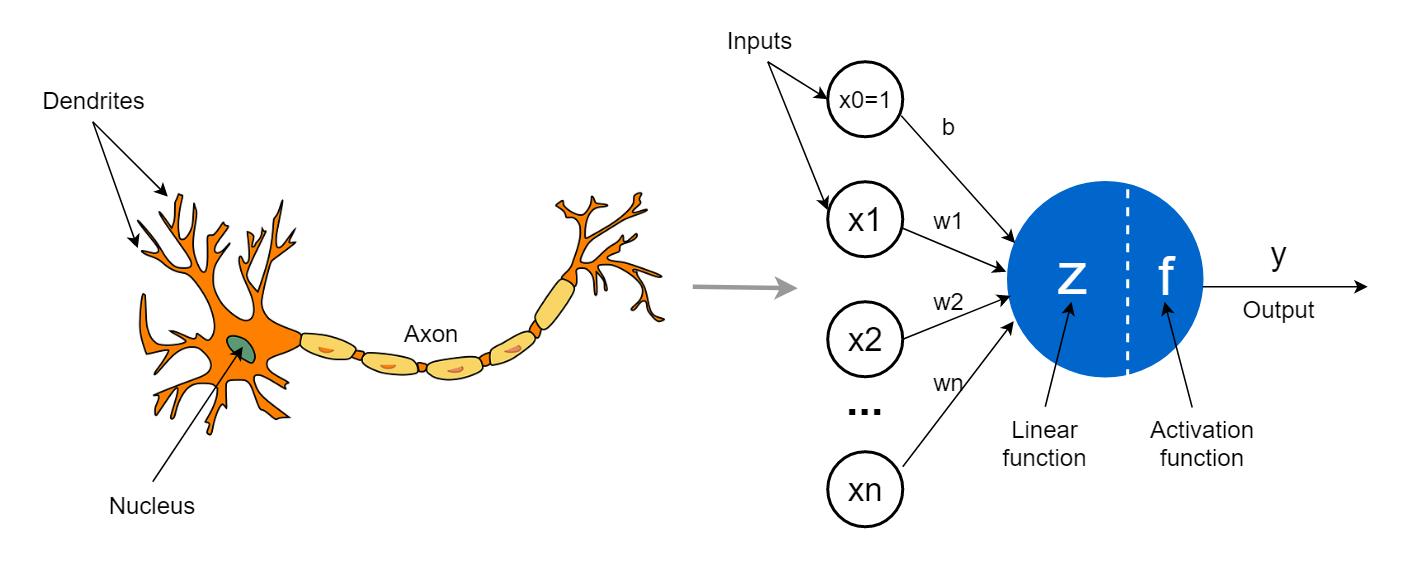
\includegraphics[width=0.75\textwidth]{neuron_vs_ann.png}
    \caption{Biological neuron vs. Artificial neuron structure.\cite{ghosh2020perceptron}}
    \label{fig:neuron_vs_ann}
\end{figure}

A typical neural network for noise cancellation consists of the following components:
\begin{itemize}
    \item \textbf{Input layer:} Receives the noisy speech signal (e.g., a time-domain waveform or its spectrogram).
    \item \textbf{Hidden layers:} Perform nonlinear transformations to extract key features and patterns from the input. These layers may include convolutional, recurrent, or fully connected neurons depending on the network architecture.
    \item \textbf{Output layer:} Produces the denoised speech signal by mapping the learned features back to the clean signal domain.
\end{itemize}

The network is trained using pairs of clean and noisy audio samples. It gradually learns to reduce the difference between its predicted output and the actual clean signal. Once trained, the model can take in new noisy speech and output a cleaner version. This learning-based approach allows neural networks to adapt to complex noise patterns, often performing better than traditional signal processing methods in real-world situations.

\section{Machine Learning}
\label{sec:machine_learning}

Machine learning (ML), a subset of artificial intelligence (AI), focuses on developing algorithms that enable systems to learn patterns from data and make decisions without being explicitly programmed. In speech enhancement, ML has enabled the design of specialised neural network architectures capable of recovering clean speech from noisy inputs. One widely used architecture is the \textit{autoencoder}, which learns to reconstruct its input via a compressed latent representation \cite{azarang2020review}.

\begin{figure}[h]
    \centering
    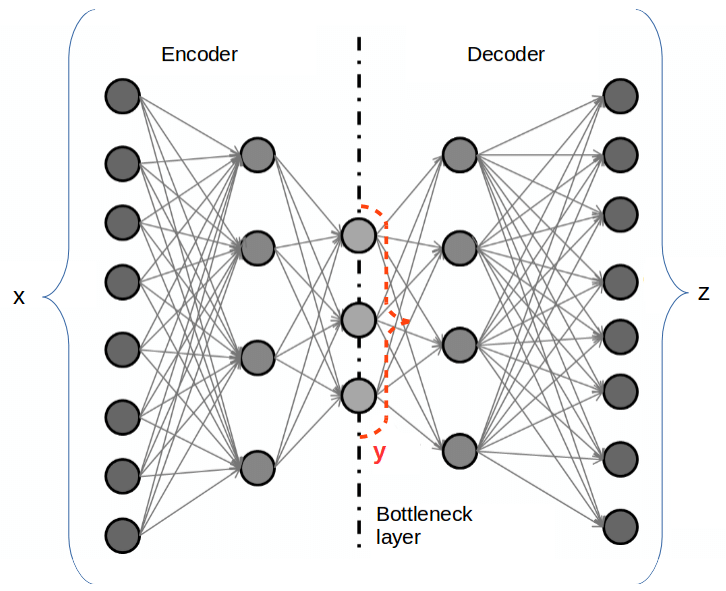
\includegraphics[width=0.5\textwidth,keepaspectratio]{autoencoder.png}
    \caption{\label{fig:autoencoder} Block diagram of an autoencoder architecture \cite{vachhani2017dae}.}
\end{figure}

An autoencoder consists of two main components: an encoder and a decoder. The encoder compresses the input signal \(x\) into a low-dimensional latent space by passing it through convolutional, pooling, or fully connected layers. A central \textit{bottleneck} layer enforces this compression, encouraging the model to retain only the most salient features—such as speech structure—while discarding irrelevant noise.

The decoder then reconstructs the signal \(y\) from the latent representation, typically using upsampling, transposed convolutions, or dense layers in a mirrored arrangement. The objective is to recover the clean speech with minimal reconstruction error.

Autoencoders are trained using paired datasets of noisy and clean speech. During training, the noisy input is passed through the network, and the output is compared to the clean reference. The model is optimised to minimise the difference—typically using a loss function such as Mean Squared Error (MSE) or Mean Absolute Error (MAE).

\begin{figure}[h]
    \centering
    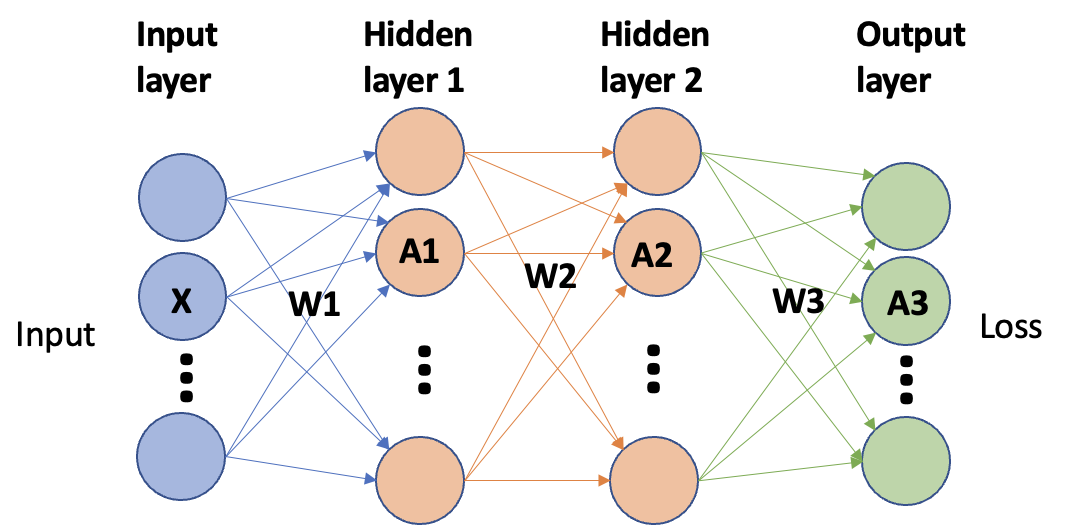
\includegraphics[width=0.5\textwidth,keepaspectratio]{weigths.png}
    \caption{\label{fig:weigths} Loss and weight update process in an autoencoder \cite{epoch2021}.}
\end{figure}

Training proceeds iteratively. A forward pass generates an output, and the loss function quantifies the error. This error is then propagated backward through the network via backpropagation to compute gradients, which are used to update the model’s weights using optimisers like Stochastic Gradient Descent (SGD) or Adam. This cycle continues for many epochs until convergence.

Recent advances have introduced more robust architectures. For example, Kim et al.~\cite{kim2024residual} proposed a residual-attention Gated Linear Unit (GLU) model for end-to-end (E2E) speech enhancement. Their model outperformed SOTA methods such as FAIR-Denoiser and CleanUNet across a wide SNR range (0–15 dB), showcasing the effectiveness of modern ML approaches.

Evaluation metrics such as SNR, PESQ, STOI, and MSE—used in these studies—will also be used in this project to assess and compare both classical and ML-based denoising systems. These metrics are discussed in detail in Chapter~\ref{chp:evaluation}.

\graphicspath{{content/chapters/4_specification/figures/}}
\chapter{Specification}
\label{chp:specification}

This chapter outlines the core setup for the project. It begins by examining the dataset’s structure and characteristics, which influence how data is preprocessed and formatted for input to the model. This is followed by a summary of the system-level requirements, including the development environment, training hardware, and memory constraints. Together, these define the context for the design and implementation decisions presented in subsequent chapters.

\section{Dataset Exploration}
\label{sec:dataset_exploration}

A key aspect of defining the system specifications is understanding the dataset used. This project employs an open-source dataset titled \textit{“Noisy speech database for training speech enhancement algorithms and TTS models”}, made available by the University of Edinburgh through its \textit{DataShare} repository~\cite{edinburghdataset}. The dataset is released under the Creative Commons Attribution 4.0 International License~\cite{ccby4}.

\url{https://datashare.ed.ac.uk/handle/10283/2791}

\begin{figure}[H]
    \centering
    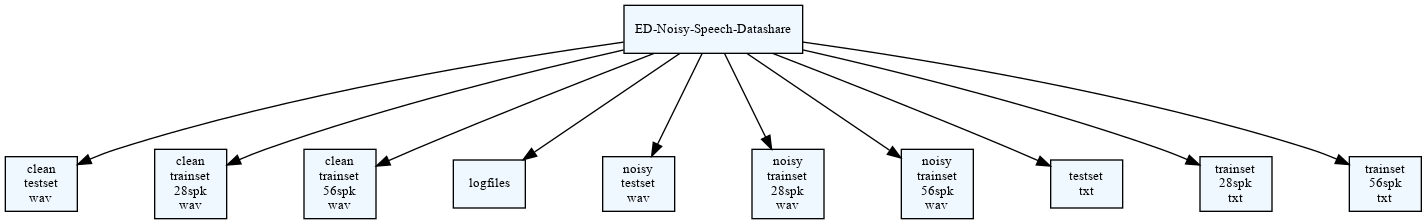
\includegraphics[width=1.0\textwidth]{dataset_structure.png}
    \caption{Dataset Tree Structure}
    \label{fig:dataset_structure}
\end{figure}

As shown in Figure~\ref{fig:dataset_structure}, the dataset is organized into three main subsets: a test set, a 28-speaker training set, and a 56-speaker training set. Each subset includes folders for transcripts, clean speech, and noisy speech shown in Figure~\ref{fig:sample_waveform_and_transcript}. Files are aligned by index across these folders, ensuring parallelism between clean and noisy samples. However, the file numbering is not continuous, with gaps in the sequence.

\begin{figure}[H]
    \centering
    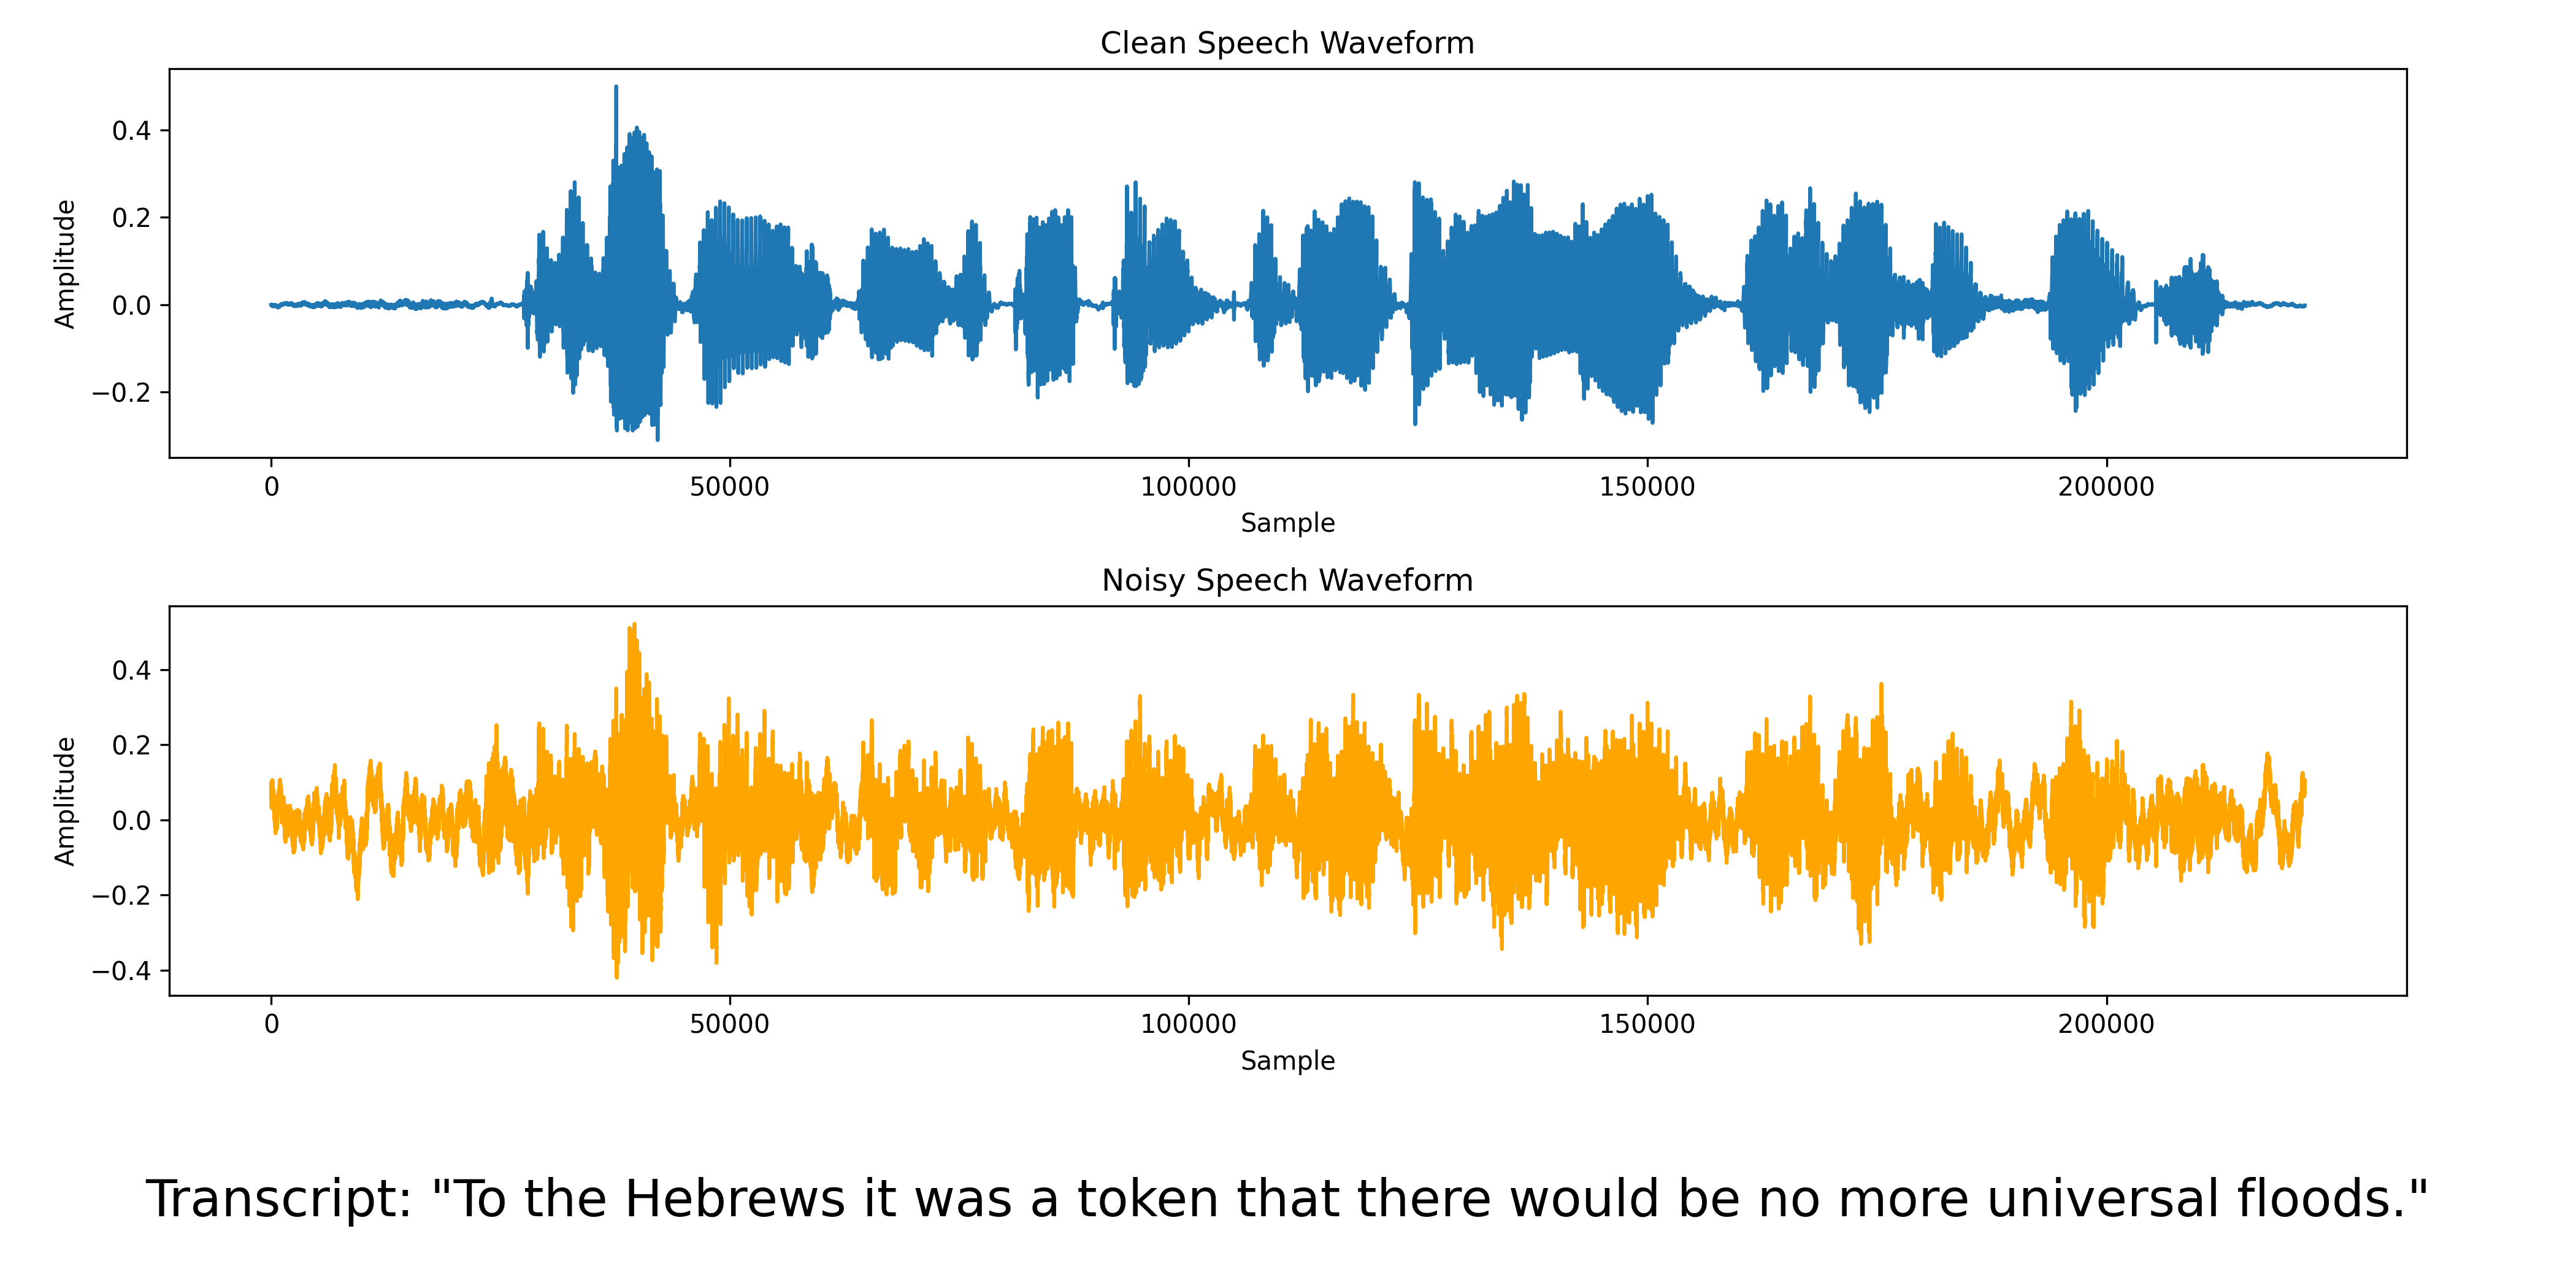
\includegraphics[width=0.8\textwidth]{sample_waveform_and_transcript.png}
    \caption{Example of a Clean, Noisy Speech Sample and its Transcript}
    \label{fig:sample_waveform_and_transcript}
\end{figure}

All audio files are in \texttt{.wav} format and sampled at 48~kHz. Clip lengths vary, which significantly impacts how data is batched and fed into the model. The dataset contains no corrupted files, and the total download size was approximately 15~GB.

\section{System Specification}
\label{sec:system_specification}

Given the computational demands of training neural networks, this project was developed and executed remotely on the University of Malta’s Interfacing Lab servers, accessed via \gls{ssh}. These machines are equipped with NVIDIA GeForce RTX 3060 GPUs, which are suitable for deep learning workloads. However, GPU memory limitations required careful control of training parameters, including batch size, model depth, and the number of epochs.

The development environment was based on \gls{vscode}, with assistance from GitHub Copilot for improved coding efficiency. Early experiments and module testing were conducted in Jupyter notebooks, which were later consolidated into a single modular Python application. This modular structure allows for separation of data preprocessing, model training, evaluation, and inference, improving maintainability and extensibility.

The final output of the system is a trained model checkpoint, which can be used for inference on new audio data. The model is compatible with industry-standard frameworks such as TensorFlow and PyTorch and is designed to be portable across machines. This enables future deployment on embedded boards or other constrained platforms for real-time speech enhancement.


\graphicspath{{content/chapters/5_design/figures/}}
\chapter{Desing}
\label{chp:design}

\section{System Design}
\label{sec:system_design}

The overall system design is modular, enabling seamless integration of different components and allowing for future extensibility. The system is divided into three main pipelines: training, denoising, and hyperparameter tuning. Each pipeline is implemented as a collection of functions with their respective parameters and outputs. These pipelines are coordinated through the \texttt{main.py} file, which serves as the entry point for the entire application.

All helper modules are organized under a \textit{Utils} folder, which contains essential functionality for dataset handling, model architecture definitions, training routines, denoising logic, and hyperparameter tuning. Additionally, a central configuration file, \texttt{config.py}, is located outside the \textit{Utils} folder near the \texttt{main.py} file. This file manages all the project’s parameters in the form of a dictionary, providing a centralized and easily modifiable interface. This approach enhances usability, allowing users to modify settings in one place and execute the pipeline directly through the main script.

A brief overview of the key files in the \textit{Utils} folder is provided below:

\begin{itemize}
    \item \texttt{dataset.py}: This file defines all dataset classes used in the project. These are implemented as PyTorch \texttt{Dataset} objects and support different strategies for handling variable-length audio inputs, as discussed in Section~\ref{sec:variable_length_handling}. This module also includes the definition of the \texttt{BucketSampler} class, which groups audio files of similar lengths to minimize padding and improve training efficiency. Additionally, it defines the \texttt{pto\_collate} function for batch collation and the \texttt{visualize\_dataset\_padding} function for visualizing the padding distribution in the dataset.
    
    \item \texttt{model.py}: This file defines all model architectures used in the project. Each model is implemented as a class inheriting from PyTorch’s \texttt{nn.Module}. Separating model definitions into their own module helps maintain a clean pipeline and facilitates experimentation with different architectures and hyperparameters.

    \item \texttt{train.py}: This file contains all functions related to model training, including the training loop, validation logic, and final evaluation. The training pipeline supports input from all three datasets defined in \texttt{dataset.py}, providing flexibility in training under different input-handling strategies. The modular design enables simple experimentation with alternative training setups and parameters.

    \item \texttt{denoise.py}: This module handles the denoising process and post-training evaluation. It follows a structure similar to the training pipeline but focuses on inference and metric computation. It supports both dataset-wide evaluation and single-sample inference. Additionally, this module allows the user to apply either of the two classical methods to the noisy input for comparison purposes, producing corresponding evaluation metrics.

    \item \texttt{classical.py}: This file implements traditional signal processing-based denoising algorithms used as baselines. These methods are implemented as standalone functions that take noisy waveforms as input and return denoised outputs. Where applicable, established libraries are used to implement these classical methods to avoid re-implementing known algorithms from scratch.

    \item \texttt{optuna.py}: This module handles hyperparameter tuning using the Optuna framework. It defines an optimization function that takes the training and validation datasets and returns the best-performing hyperparameter configuration. Due to the high memory requirements of certain models and datasets, this tuning pipeline is still being optimized for improved stability and efficiency.
\end{itemize}

\section{Variable Length Handling}
\label{sec:variable_length_handling}

For this project, only the clean and noisy pairs of audio files from the dataset are required — the transcript text files are ignored, as they are not relevant to the task. However, it is worth noting that such transcripts are highly valuable in other applications, such as training text-to-speech or speech recognition models.

As highlighted in the dataset analysis in Section~\ref{sec:dataset_exploration}, the audio files vary in length. This poses a challenge for model training, as batch processing requires input tensors to have consistent dimensions.

To address this, several algorithms for handling variable-length audio inputs were explored. The most basic approach involves padding each audio file to match the length of the longest sample in the batch, typically by appending zeros to the end of shorter files. While this method is simple, it has significant drawbacks: excessive padding introduces unnecessary data that may act as noise during training, making it harder for the model to learn effectively. The greater the variation in input lengths, the more padding is required — which can negatively impact overall training performance.

\begin{figure}[h]
    \centering
    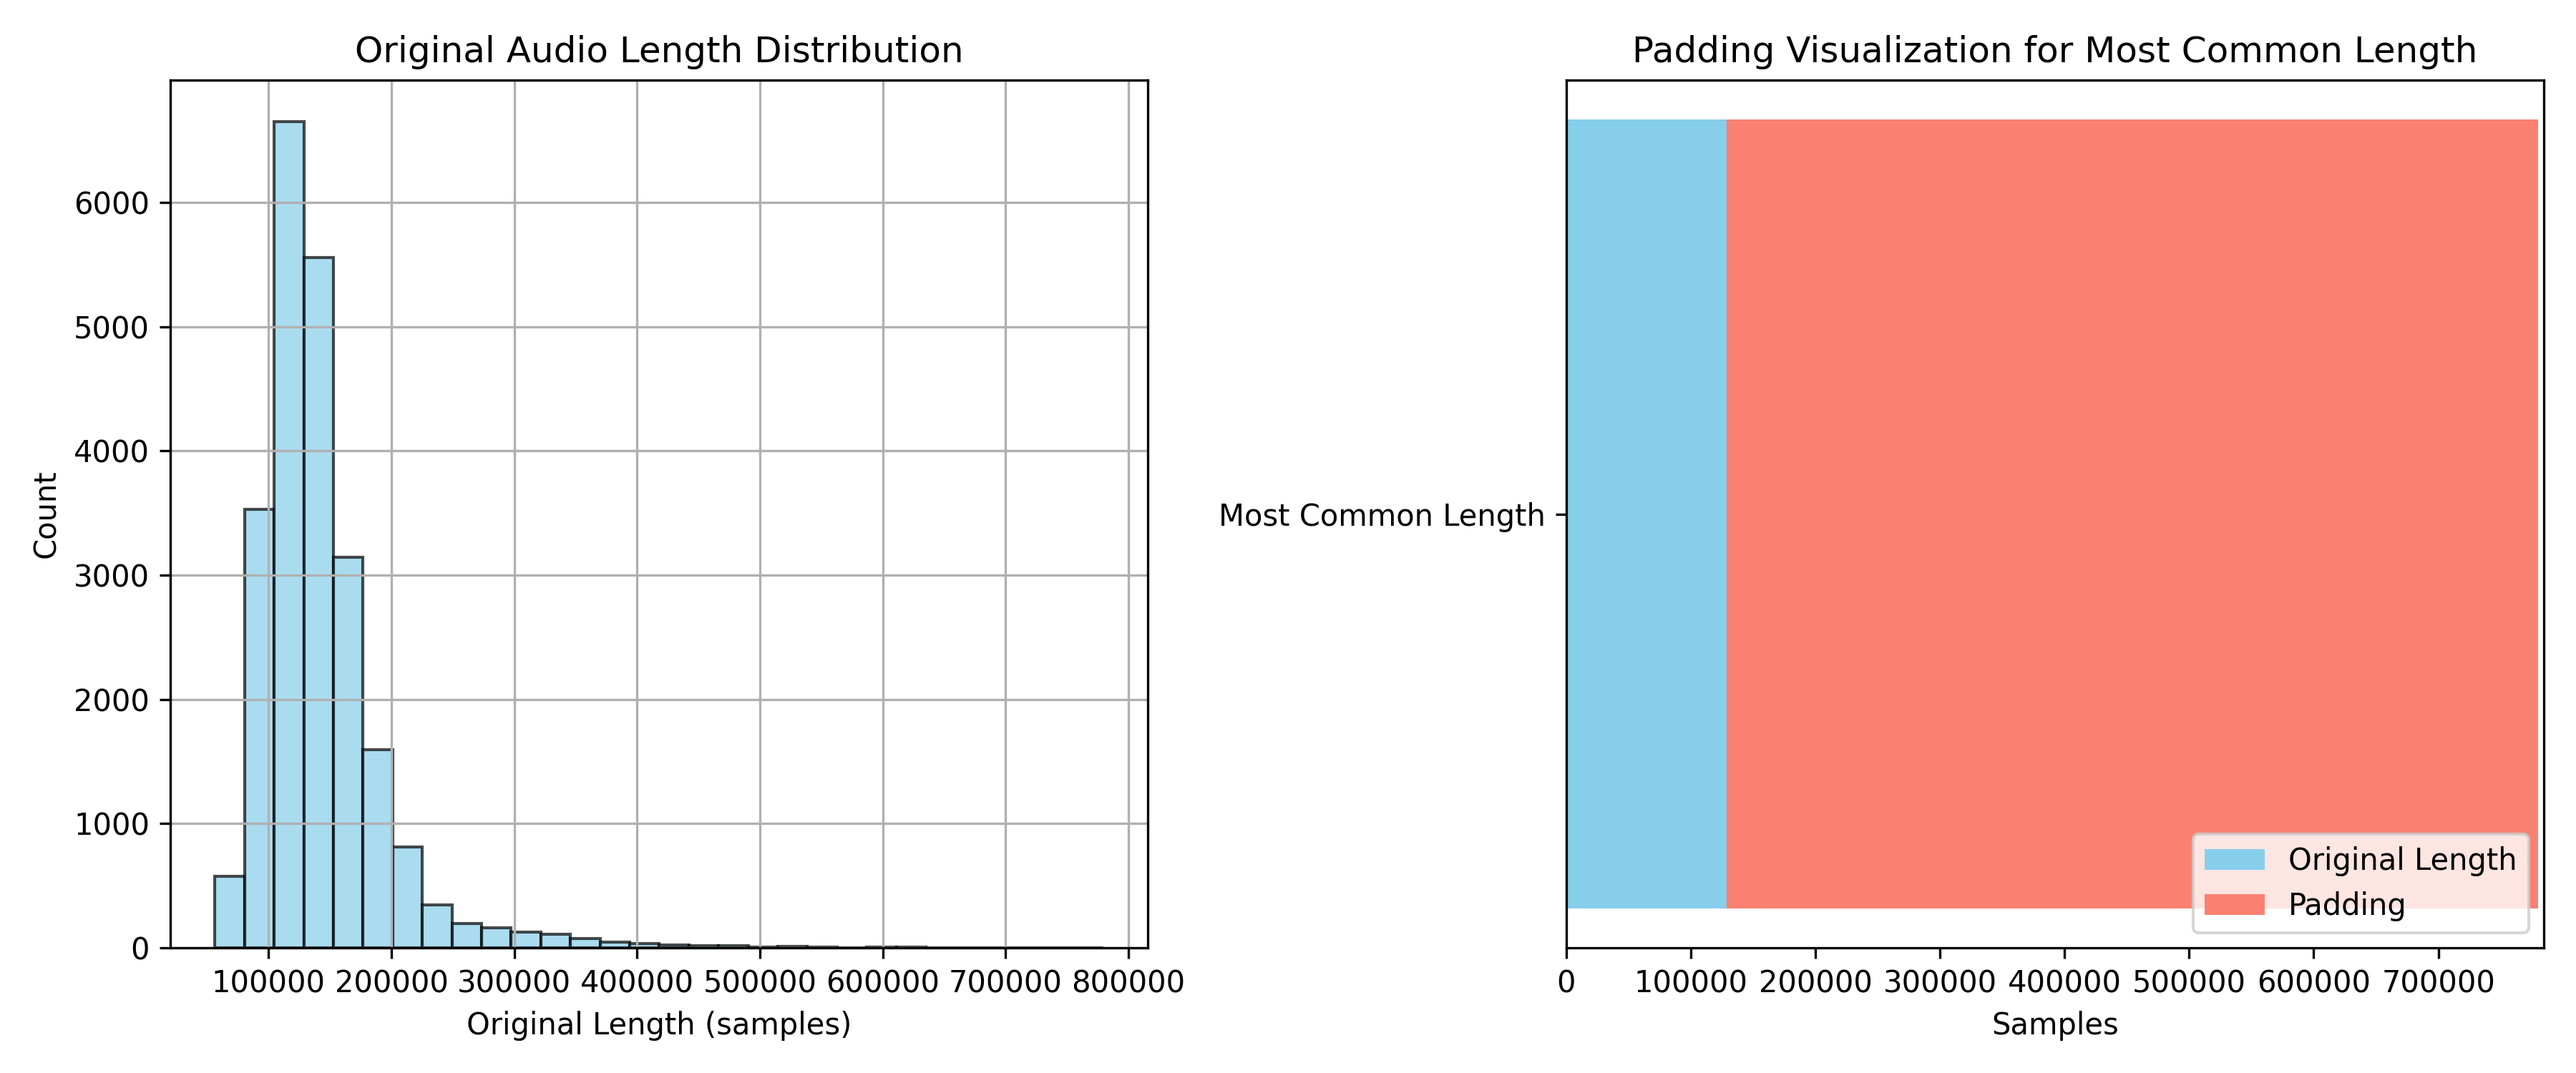
\includegraphics[width=\textwidth,keepaspectratio]{max_padding.png}
    \caption{\label{fig:max_padding}Illustration of maximum-length padding.}
\end{figure}

As shown in Figure~\ref{fig:max_padding}, the most common audio length is padded so heavily that the padding exceeds the actual content. This is far from ideal. To mitigate this issue, three different padding strategies were implemented. Each method aims to reduce the impact of excessive padding on model performance.

The first method is \textit{Static Bucketing}, which groups audio files into predefined fixed-length buckets. Building on this, the second method, \textit{Dynamic Bucketing}, creates buckets dynamically based on the distribution of audio lengths, offering a more adaptive grouping approach. The third and final method, inspired by a research paper~\cite{yoon2020pto}, proposes a simple, distortion-free technique for handling variable-length sequences through a combination of padding, truncation, and output truncation.

All three methods were implemented for testing and evaluation. Their role in the system design is critical, as they help ensure that the model can learn effectively without being hindered by dimensional mismatches or excessive zero-padding. Further details on the implementation of these methods are provided in Chapter~\ref{chp:implementation}, and their impact on model performance is discussed in Chapter~\ref{chp:evaluation}.

\section{Model Architecture}
\label{sec:model_architecture}

The model architecture is the highlight of the system design. It is the core component that determines how the system processes input data, how hidden layers and their connections are defined, and how the final output is generated. The modular design of the project as a whole facilitates the exploration of various model architectures. The main structure for speech enhancement models has already been introduced in Chapter~\ref{chp:literature_review}. With the concept of autoencoders being well-established in the literature, the most basic model defined in this work is a convolutional neural network (CNN) autoencoder.

\subsection{Convolutional Autoencoder (CNN)}

The CNN model implemented in this project serves as the baseline architecture. It is designed as a basic encoder-decoder model that operates directly on the real and imaginary components of the spectrogram, which are concatenated into a two-channel input. The encoder compresses the input using a series of convolutional layers and ReLU activations, reducing spatial dimensions while increasing the feature depth. A bottleneck layer captures the most salient features, followed by a decoder made of transposed convolutions that upsample the compressed representation back to the original shape.

The final output layer uses a \texttt{tanh} activation to constrain the values between -1 and 1, matching the typical range of normalized spectrogram values. The output is then split back into separate real and imaginary components. This basic structure allows the model to learn an end-to-end mapping from noisy spectrogram input to a denoised output while maintaining the shape consistency required for spectrogram inversion.

While simple, this model is critical for establishing a performance baseline and ensuring that the data pipeline, loss function, and inference process are correctly implemented.

\subsection{U-Net Architecture}

A U-Net is a type of convolutional neural network (CNN) commonly used for image segmentation tasks due to its effectiveness in preserving spatial information through skip connections. It is particularly well-suited for scenarios where both global context and fine-grained local detail are important — making it a strong candidate for spectrogram-based speech enhancement.

In this project, the U-Net architecture has been adapted to work with complex-valued spectrograms. Both the input and output consist of two channels representing the real and imaginary parts of the signal. The encoder compresses the input through multiple convolutional layers, each followed by group normalization and PReLU activations. The decoder performs the inverse operation using transposed convolutions, reconstructing the output with the help of skip connections from the encoder layers. These skip connections are aligned using bilinear interpolation to ensure matching dimensions, which is essential due to the varying spatial resolution after convolutional operations.

Compared to the basic CNN, the U-Net provides a deeper architecture with significantly better capacity for modeling both local patterns and long-range dependencies in the spectrogram. Its design allows for improved gradient flow and better reconstruction of fine detail in the denoised output.

\subsection{Conv-TasNet Architecture}

The Conv-TasNet is a convolutional, time-domain-based architecture originally proposed for speech separation. It avoids recurrence entirely by using stacked temporal convolutional networks (TCNs) to model long-term dependencies. In this project, the Conv-TasNet has been adapted for the frequency domain by operating on 2D spectrogram data, with two channels corresponding to the real and imaginary parts.

The architecture begins with an encoder that applies a convolutional transformation to the input spectrogram, projecting it into a higher-dimensional feature space. This is followed by a separation network composed of multiple stacks of dilated residual blocks, forming the TCN. These blocks use increasing dilation rates to capture long-range dependencies while maintaining efficient computation. Each residual block contains two convolutional layers, PReLU activation, and batch normalization, with residual connections ensuring stable gradient flow.

The decoder then transforms the processed features back into a two-channel spectrogram through another convolutional layer. To maintain shape consistency, both the residual blocks and the decoder truncate or interpolate the output as needed.

This architecture offers a high degree of temporal modeling while maintaining the advantages of convolutional efficiency. It serves as the most complex and expressive model evaluated in this project and is intended to compete with state-of-the-art enhancement techniques.

\subsection{Summary}

All three architectures were implemented within a unified framework that supports modular experimentation. Each model accepts and outputs two-channel spectrogram data, ensuring compatibility with the complex-valued processing pipeline. The CNN serves as a foundational benchmark, the U-Net balances performance with architectural elegance, and the Conv-TasNet pushes the boundary of what is achievable with convolutional architectures in this context. Their comparative performance and trade-offs are evaluated in Chapter~\ref{chp:evaluation}.



\graphicspath{{content/chapters/6_implementation/figures/}}
\chapter{Implementation}
\label{chp:implementation}

\section{Datasets}
\label{sec:datasets}

Following Section~\ref{sec:variable_length_handling}, this section describes the dataset handling mechanisms implemented to accommodate variable-length audio signals. The custom dataset classes developed for this project inherit from PyTorch’s \texttt{Dataset} class and are used in both training and denoising pipelines. These implementations are central to managing waveform padding, STFT conversion, and batch preparation for machine learning models.

Each class implements three essential methods that are all similarly structured but differ in their approach to handling variable-length data. The \texttt{\_\_init\_\_} method initializes key parameters, constructs paths for clean and noisy speech files, and prepares required caches. Here the amount of parameter varies based on the approach as some methods require more configuration than others. The \texttt{\_\_len\_\_} method is a simple return function that provides the total number of samples in the dataset. The \texttt{\_\_getitem\_\_} method applies necessary transformations to the audio files such as mono conversion, resampling, and STFT. It also handles the padding and truncation of audio samples to ensure consistent input dimensions across batches. Real and imaginary STFT components are used as input-output pairs, ensuring a consistent format across all datasets. A critical motivation for this implementation is real-time deployment. The STFT inherently segments audio into short overlapping frames, simulating real-time input. This makes training models on STFT frames suitable for later real-time inference.

\subsection{Static Bucketing}
\label{subsec:static_dataset}

The first dataset implementation explored to address the variable-length issue and limitations of fixed-length padding is the static bucketing method. This approach uses a predefined set of bucket sizes, each corresponding to a fixed number of audio samples. In this project, sizes were derived by multiplying the sampling rate (48~kHz) by target durations (e.g., 1s, 2s, 3s), resulting in discrete, fixed-length buckets.

Each audio file is assigned to the first bucket that can fully contain it. For example, an audio clip of 2.5 seconds is assigned to the 3s bucket, since the 2s bucket is insufficient, and the 3s bucket is the next available option.

\begin{figure}[H]
    \centering
    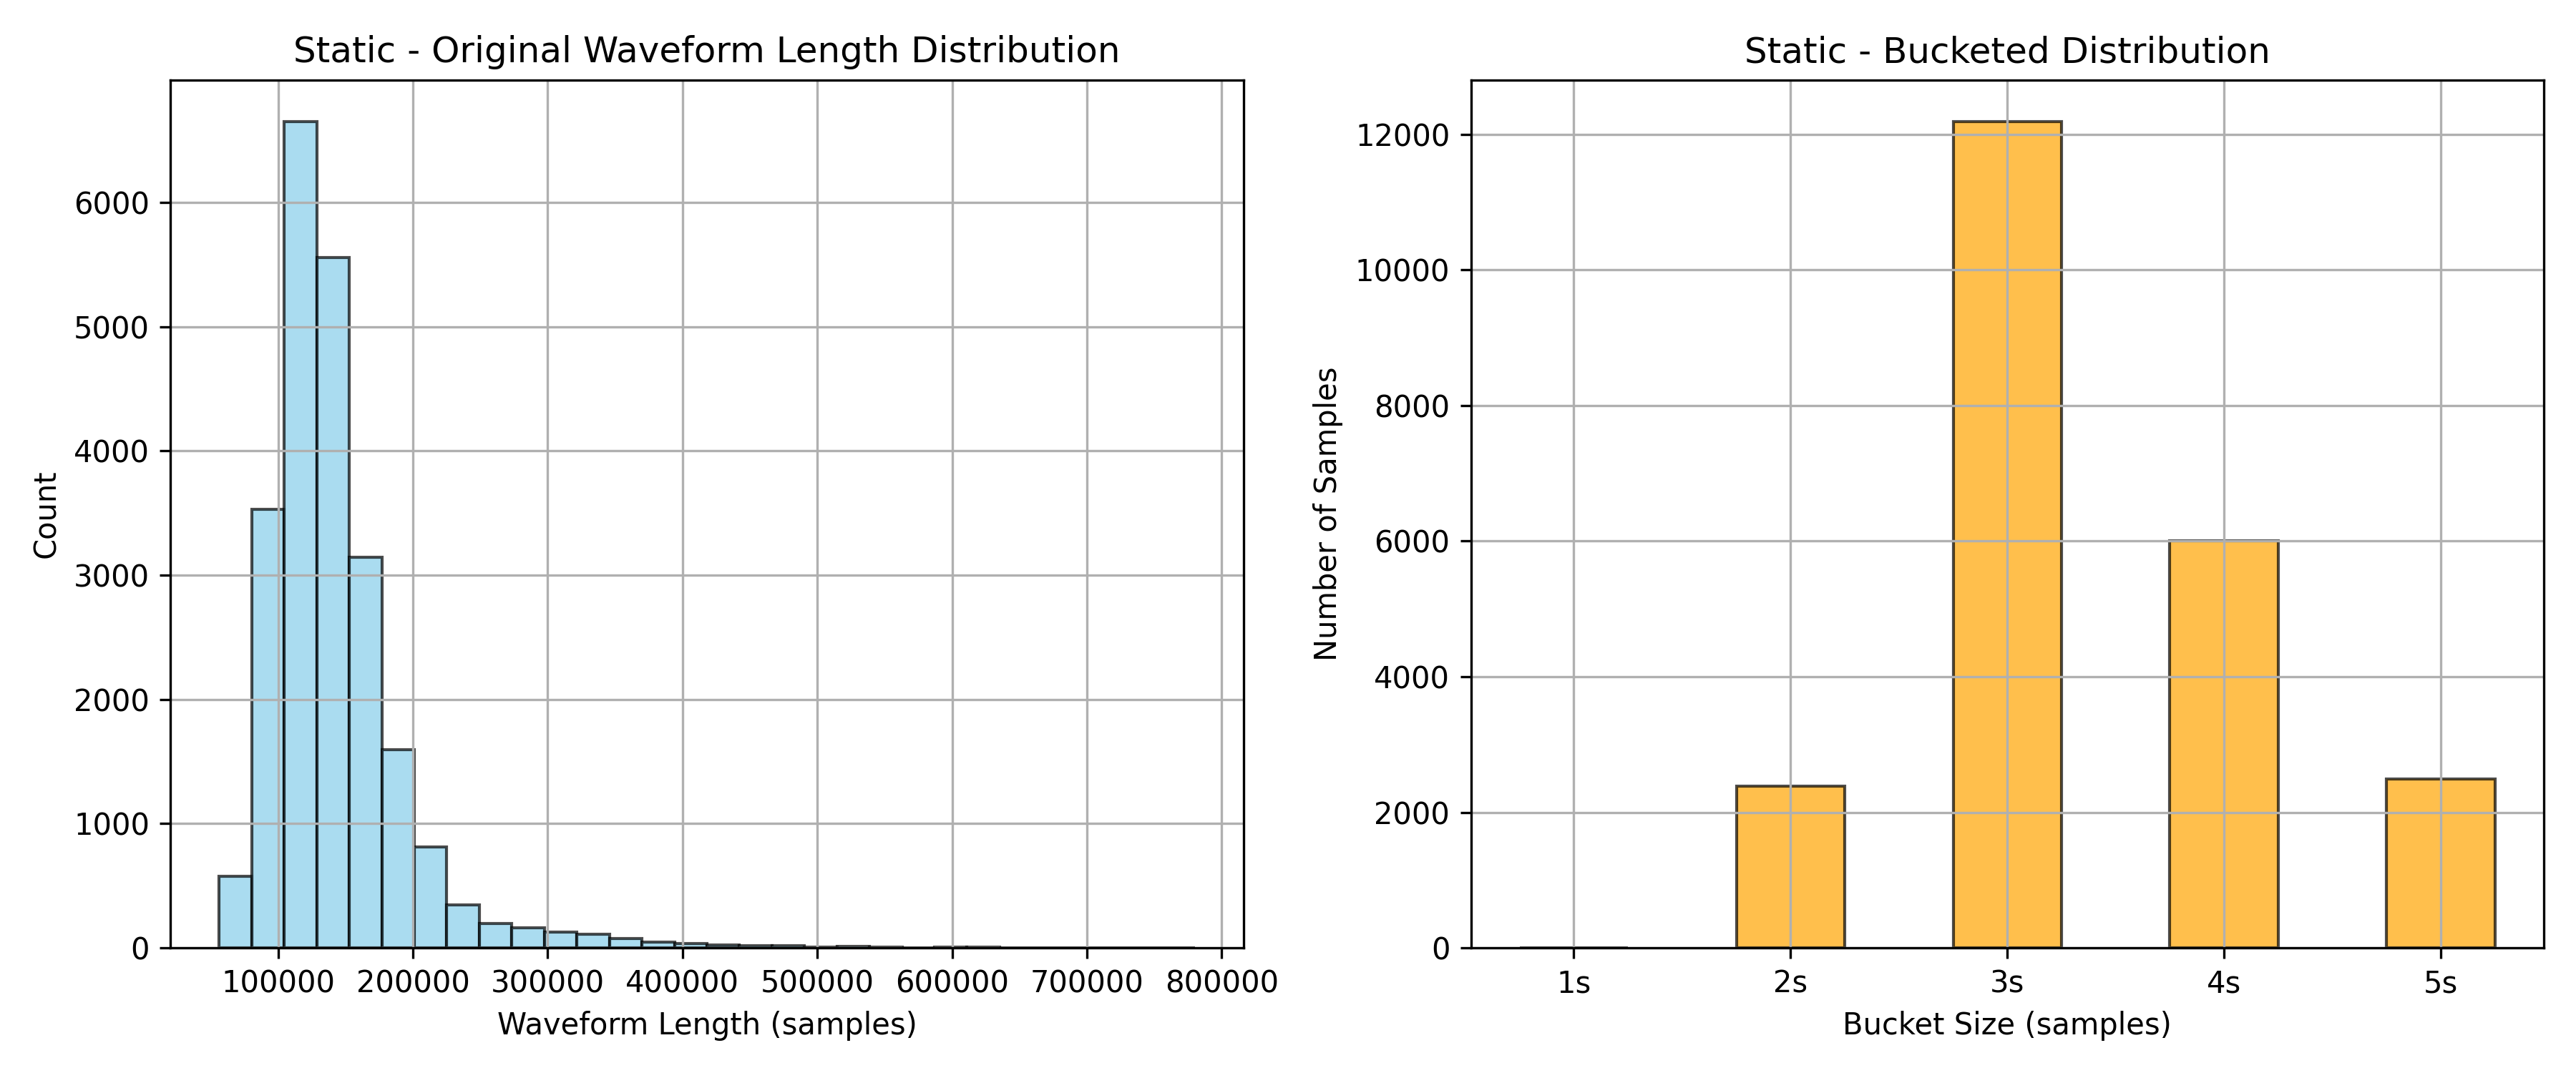
\includegraphics[width=0.9\textwidth]{static_pad.png}
    \caption{Static bucketing histogram and bucket allocation}
    \label{fig:static_pad}
\end{figure}

The \texttt{bucket\_handler} method iterates over all clean files, assigns them to buckets, and caches these assignments to avoid redundant processing in future runs. During training, a custom \texttt{collate} function pads or truncates audio waveforms to match their bucket’s target length. This guarantees consistent input dimensions within each batch, which is essential for batch-based processing in neural networks.

While static bucketing does not eliminate padding altogether, it significantly reduces the amount of excess padding compared to a naive fixed-length strategy. As shown in Figure~\ref{fig:static_pad}, most samples naturally group into the smaller buckets (3s), improving efficiency and reducing unnecessary computation.

\subsection{Dynamic Bucketing}
\label{subsec:dynamic_dataset}

The dynamic bucketing method improves upon static bucketing by adapting the bucket sizes to the actual distribution of audio file lengths. Instead of predefined durations, the method uses K-Means clustering on the waveform lengths to compute optimal bucket centers. This enables buckets that reflect the natural variance in the dataset.

During initialization, the method measures the length of each clean file and applies K-Means with a specified number of clusters (\texttt{num\_buckets}). These cluster centers become the bucket sizes, and each sample is assigned to the closest one. Like static bucketing, this assignment is cached.

\begin{figure}[H]
    \centering
    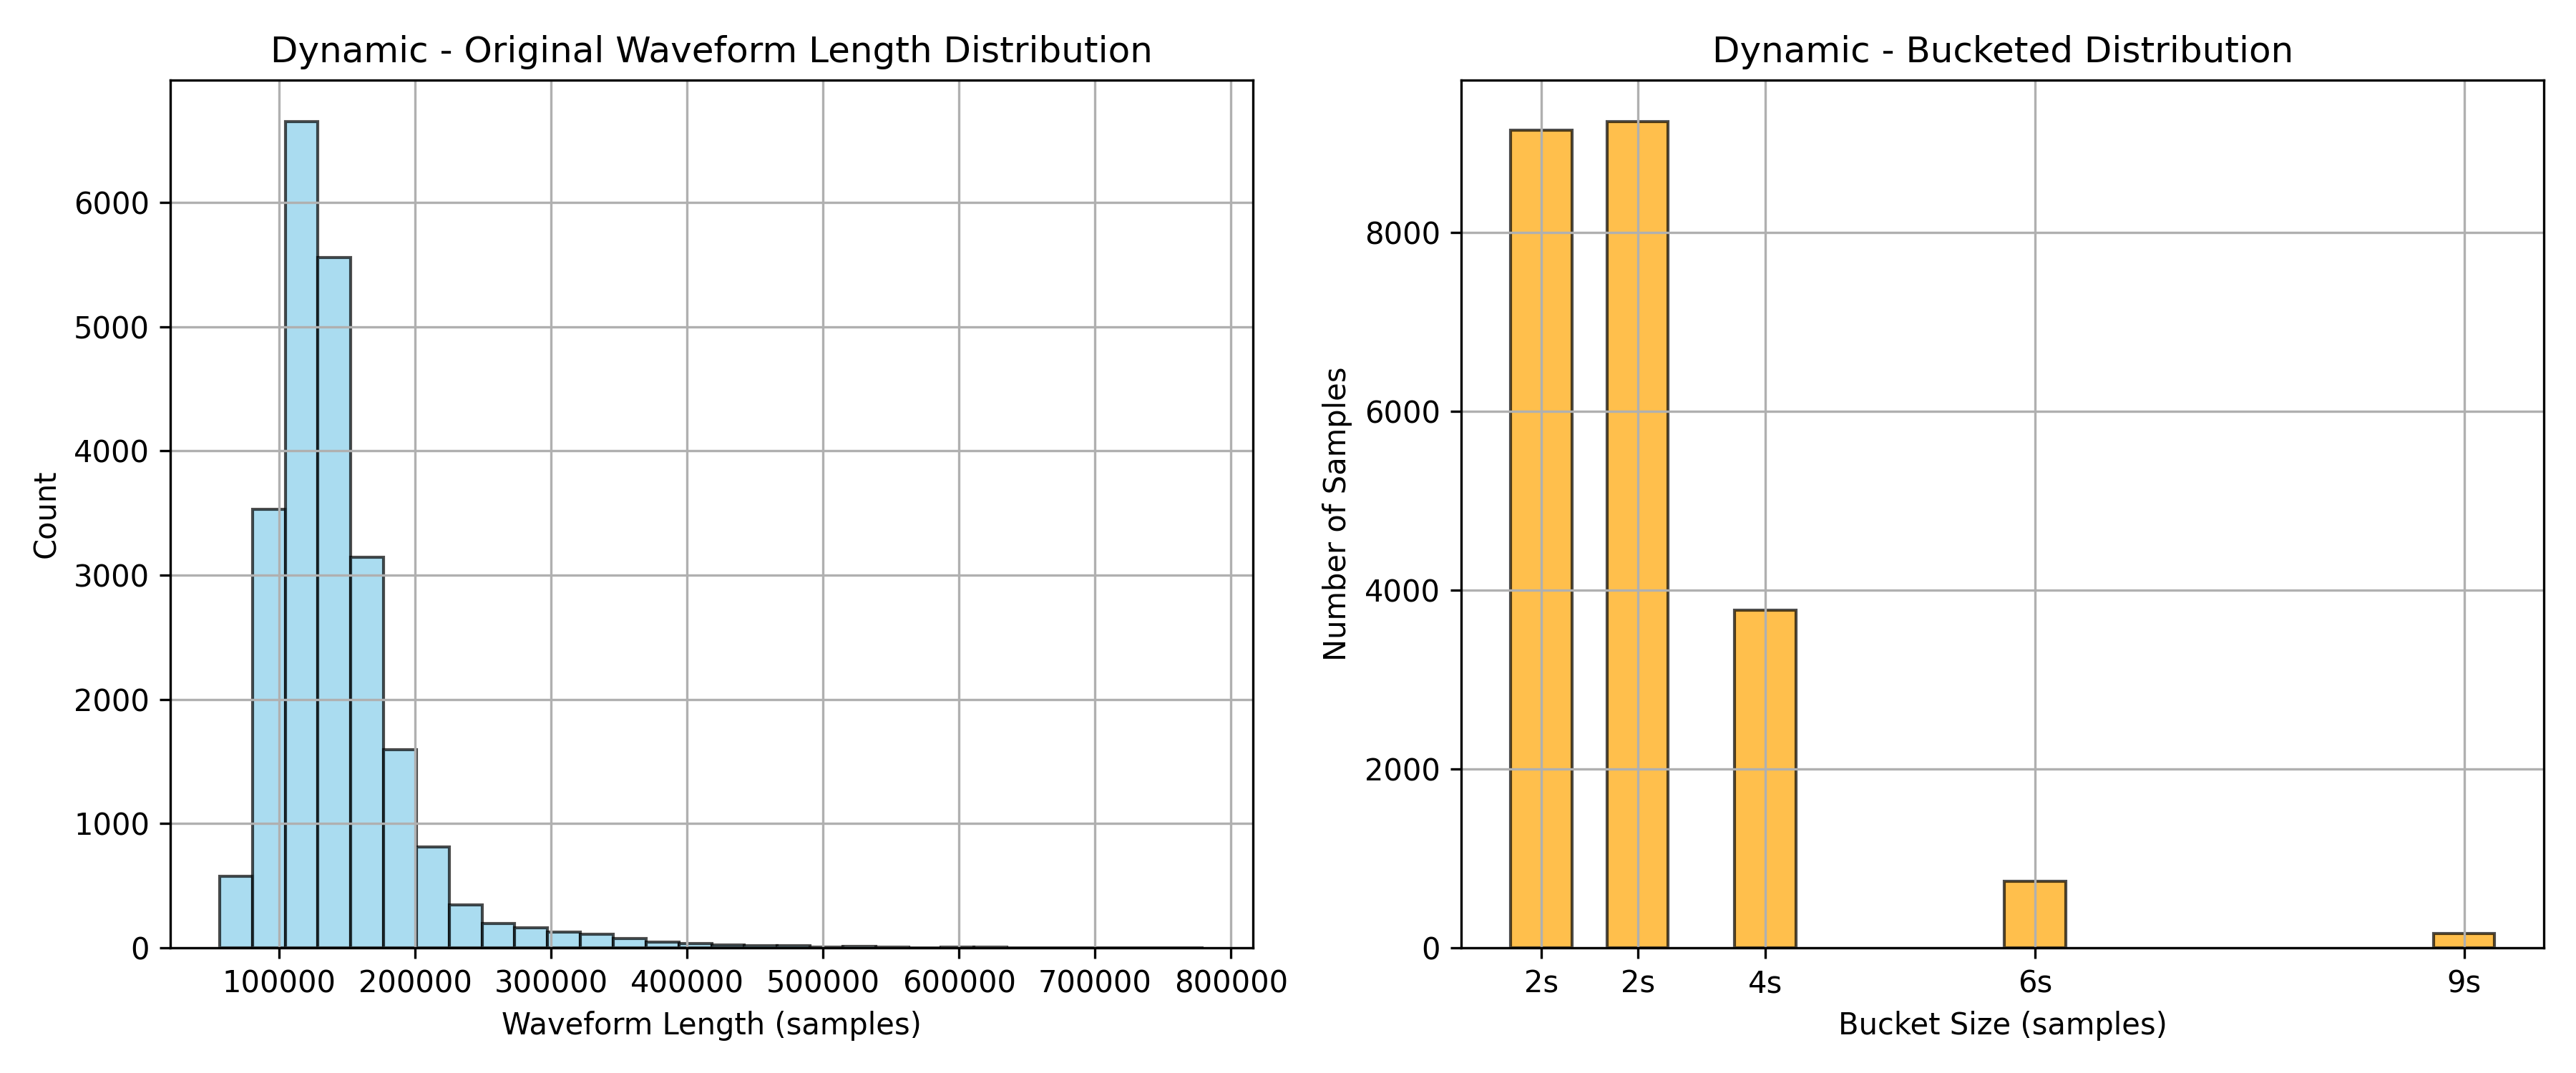
\includegraphics[width=0.9\textwidth]{dynamic_pad.png}
    \caption{Dynamic bucketing histogram and bucket allocation}
    \label{fig:dynamic_pad}
\end{figure}

The \texttt{collate} method then pads or truncates each waveform to its bucket's target size. Compared to static bucketing, dynamic bucketing leads to tighter groupings, minimizing the average amount of padding per batch. This results in better memory utilization and more efficient training.

Dynamic bucketing combines flexibility with performance, adapting to the dataset rather than imposing fixed constraints. It is particularly effective when the data contains a wide or uneven distribution of sequence lengths. When comparing dynamic to static bucketing, we observe that the dynamic method identifies two buckets around the 2-second mark that are heavily populated—clearly illustrating its ability to adapt to the underlying structure of the dataset more effectively than the fixed approach.

\subsection{Padding-Truncation Output-Truncation (PTO)}
\label{subsec:pto_dataset}

The Padding-Truncation Output-Truncation (PTO) approach avoids both fixed-length and bucketing strategies. Instead, it applies padding on a per-batch basis, using the longest sample in the batch as a reference. This ensures minimal padding while maintaining alignment within the batch.

The core idea is drawn from the work of Zhao et al.~\cite{yoon2020pto}, which proposed an output-truncation mechanism for real-time audio processing. During training, each sample is padded to match the maximum length in the batch, and its original length is stored. After inference, the output is cropped back to the original length, ensuring alignment with the unpadded input.

\begin{figure}[H]
    \centering
    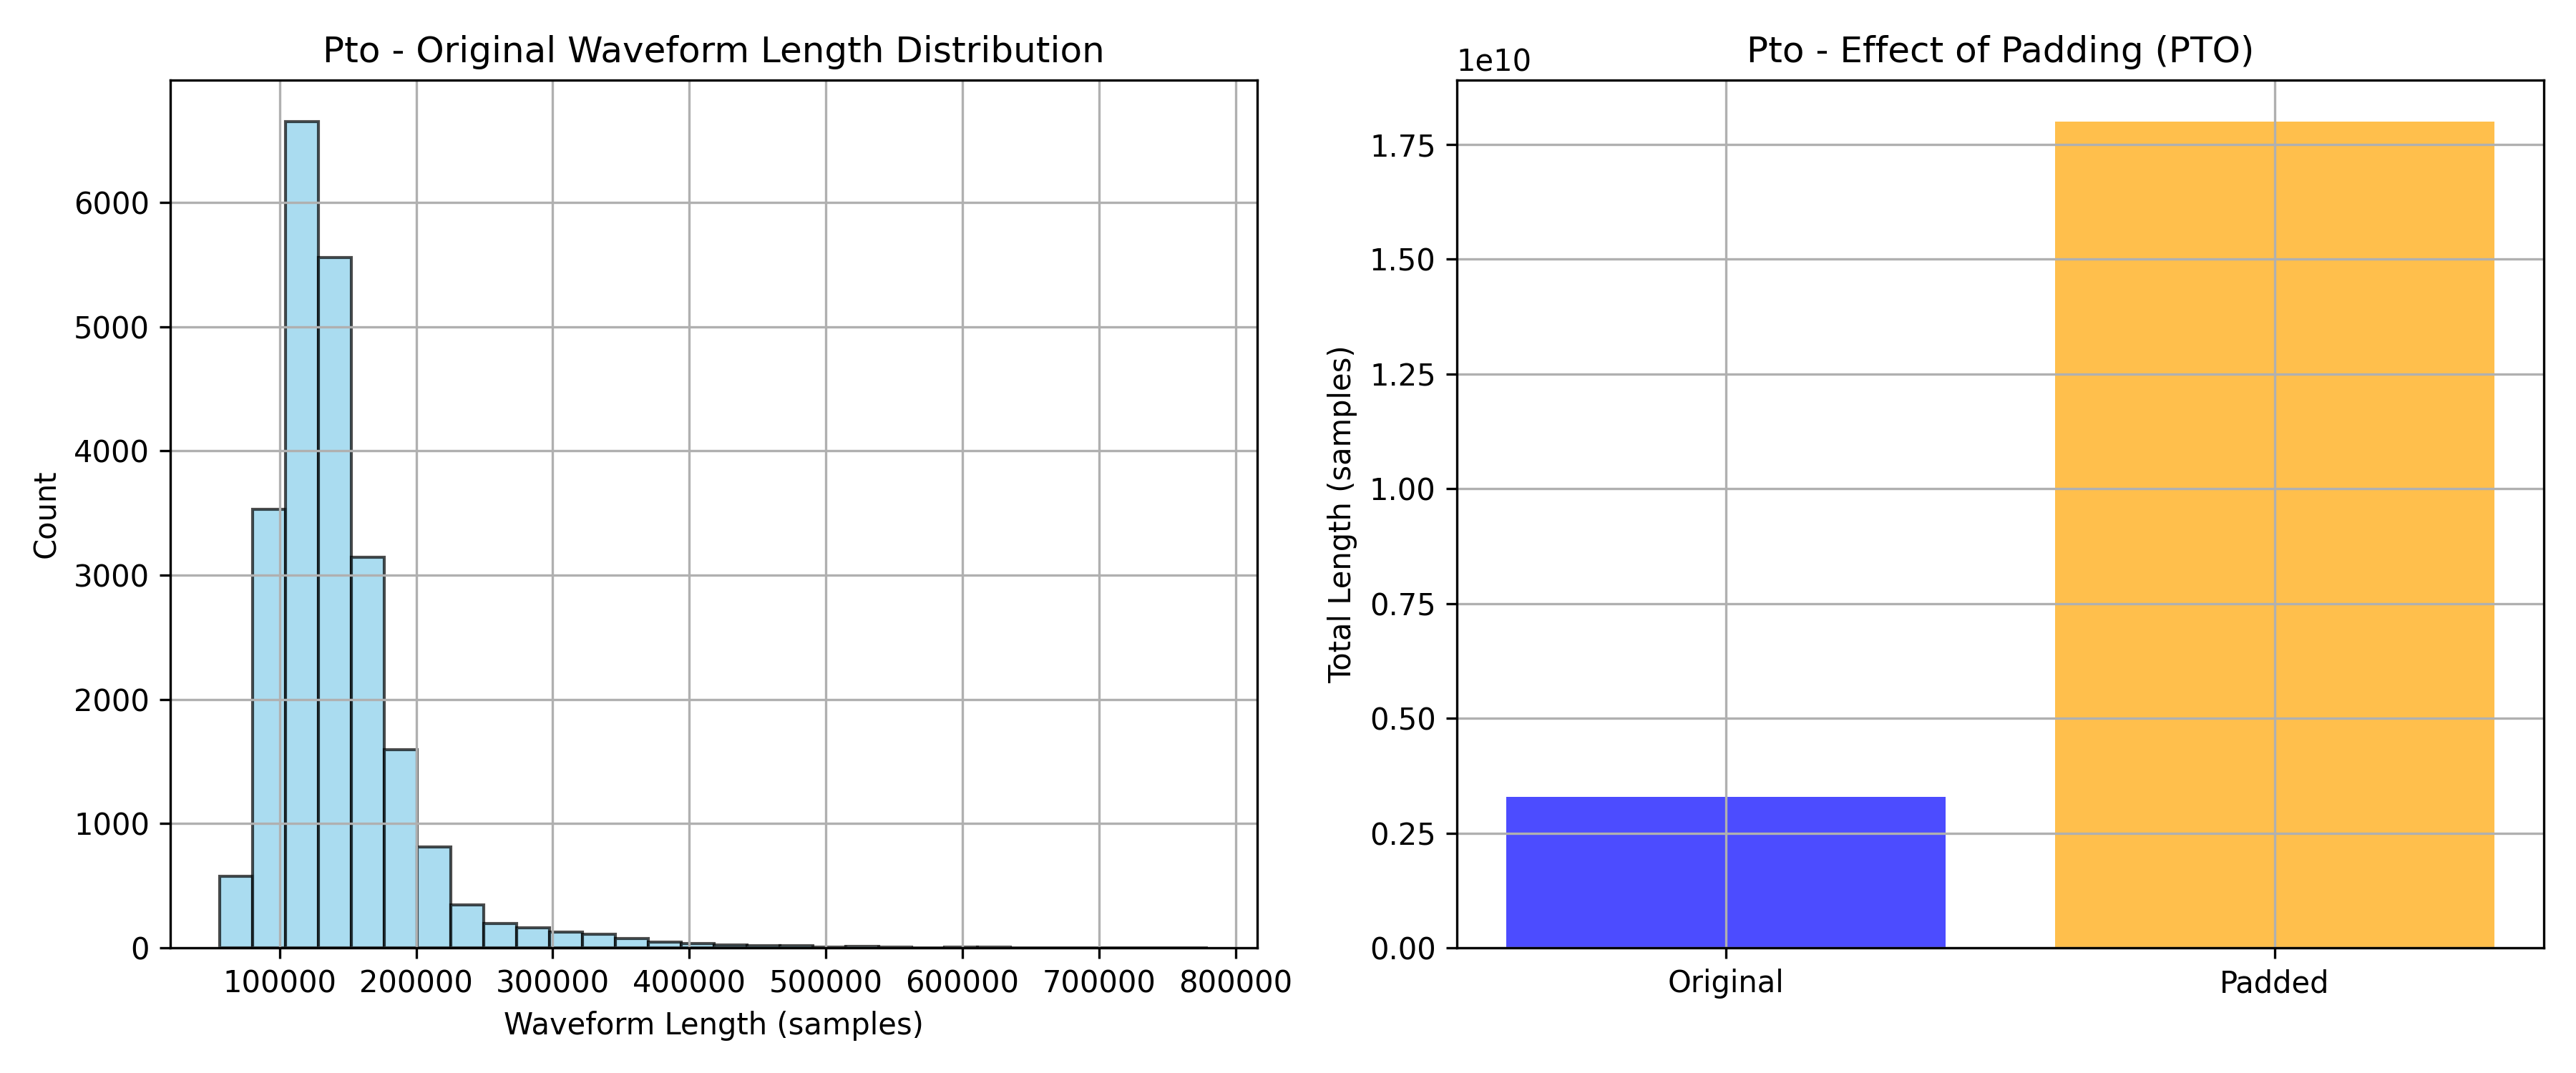
\includegraphics[width=0.9\textwidth]{pto_pad.png}
    \caption{Padding effect using the PTO method}
    \label{fig:pto_pad}
\end{figure}

In this implementation, a custom \texttt{pto\_collate} function first aligns the frequency dimension using bilinear interpolation, then pads the time axis. The model is trained on uniformly shaped tensors, but retains the ability to reconstruct clean speech at its original length, mitigating the impact of zero-padding.

The PTO method simulates real-time signal processing by training on frame-aligned STFT inputs, making it highly suitable for deployment in low-latency scenarios. Unlike bucketing methods, it does not require predefined groups or length clustering, making it the most dynamic and adaptive option in the dataset pipeline. However, it does come with its own computational overheads, as padding is still required. Furthermore, output truncation introduces an additional processing step. Although padding is mitigated at inference by truncating the output, the model is still trained on padded inputs—therefore, the cost of padding is not entirely eliminated.

\subsection{Helper Functions}
\label{subsec:helper_functions}

A few support functions are implemented to ensure that batching and visualization are handled effectively across dataset variants:

\begin{itemize}
    \item \texttt{pto\_collate}: A custom collate function used by the PTO dataset. It aligns all spectrograms along the frequency axis and pads them along the time axis, while retaining the original lengths for post-processing.
    \item \texttt{BucketSampler}: Used with static and dynamic bucketing. It ensures that batches contain only samples from the same bucket, preventing dimension mismatch during training. It randomizes batches within buckets to improve generalization.
    \item \texttt{visualize\_dataset\_padding}: A diagnostic utility that plots the distribution of original lengths and the effects of padding for each method. It provides insights into the efficiency and overhead introduced by each strategy.
\end{itemize}


\section{Out-of-Memory (OOM) Handling}
\label{sec:oom_handling}

Out-of-Memory (OOM) errors were encountered while training deeper model architectures, even with relatively small batch sizes (e.g., 4). These errors are common in GPU-constrained environments due to the increased number of trainable parameters and the large size of spectrogram tensors derived from high-resolution audio. Figure~\ref{fig:oom_error} shows a representative OOM error message encountered during training.

\begin{figure}[H]
    \centering
    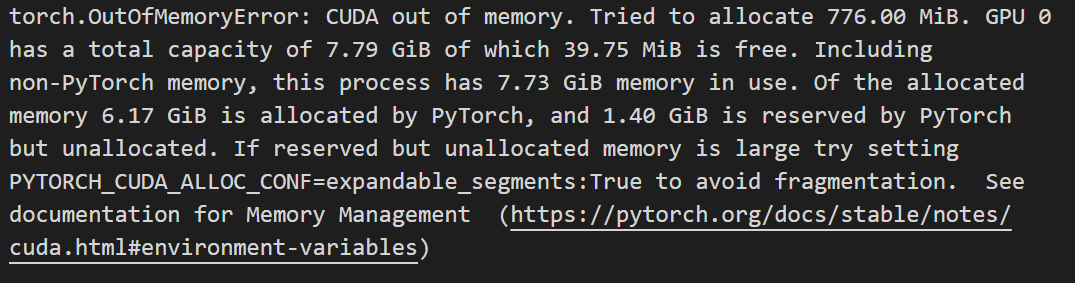
\includegraphics[width=0.8\textwidth]{oom_error.png}
    \caption{\label{fig:oom_error} PyTorch CUDA out-of-memory error message.}
\end{figure}

To address these limitations, several memory management strategies were implemented to stabilize training and enable deeper models to run within the available GPU resources. These methods also allowed the system to simulate larger batch sizes and achieve better convergence. The following techniques were used to mitigate OOM errors:

\begin{itemize}
    \item \textbf{Expandable CUDA Segments:} Before initiating training, the environment variable \texttt{PYTORCH\_CUDA\_ALLOC\_CONF=expandable\_segments:True} is set. This enables PyTorch’s new memory allocator with segment expansion, which helps alleviate fragmentation issues and allows the allocator to resize memory segments dynamically. This is the first suggestion from the PyTorch documentation for OOM errors.

    \item \textbf{Mixed Precision Training:} Automatic mixed precision (AMP) was used via PyTorch’s \texttt{autocast()} and \texttt{GradScaler}. This allows intermediate tensors to be stored in 16-bit floating point (FP16) format, reducing memory usage and increasing throughput, while maintaining model weights and gradient computations in 32-bit (FP32) for stability. Figure~\ref{fig:fp16_vs_fp32} illustrates the reduced bit-width and structure of FP16 compared to FP32, highlighting the potential for nearly half the memory usage in forward and backward passes~\cite{mindspore_mixed_precision}. This approach significantly extends the trainable capacity of a model under constrained GPU environments.

    \begin{figure}[H]
        \centering
        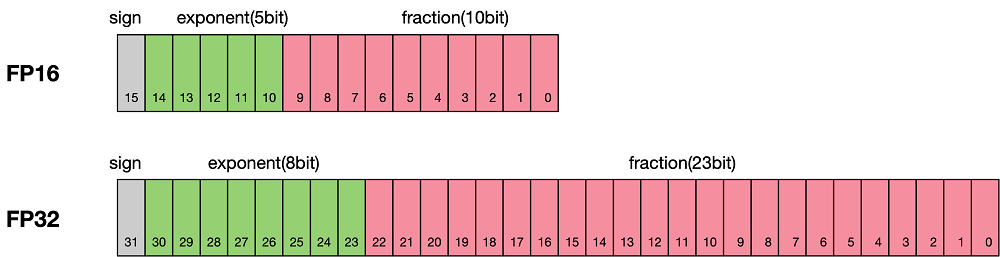
\includegraphics[width=0.9\textwidth]{fp16_vs_fp32.png}
        \caption{Comparison of memory allocation structure between FP16 and FP32 formats \cite{mindspore_mixed_precision}.}
        \label{fig:fp16_vs_fp32}
    \end{figure}

    \item \textbf{Gradient Accumulation:} Due to memory limitations that constrained the feasible batch size, gradient accumulation was employed to simulate a larger effective batch size. By accumulating gradients over multiple mini-batches and updating the model weights only every \texttt{accumulation\_steps} iterations, the training process preserves the learning dynamics of a larger batch size without exceeding memory constraints. However, directly plotting the scaled loss can result in misleading visualizations, such as those shown in Figure~\ref{fig:scaled_loss}. Where the logged values may appear artificially small or flat. To mitigate this, the raw (unscaled) loss is computed and stored separately before scaling. This ensures that both training and validation loss curves accurately reflect model performance trends, even when gradients are accumulated across steps.

    \begin{figure}[H]
        \centering
        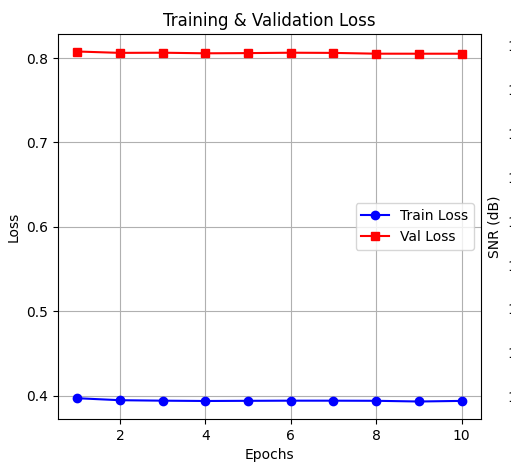
\includegraphics[width=0.6\textwidth]{scaled_loss.png}
        \caption{Plot Result When Scalling Losses}
        \label{fig:scaled_loss}
    \end{figure}


    \item \textbf{Manual Memory Management:} To ensure memory is cleared between epochs and reduce fragmentation, memory cleanup routines are explicitly called at the start of every epoch: \texttt{gc.collect()}, \texttt{torch.cuda.empty\_cache()}, and \texttt{torch.cuda.reset\_peak\_memory\_stats()}. This manual intervention is particularly beneficial in a shared GPU setting, where residual allocations from other users or previous epochs may linger.

    \item \textbf{Gradient Clipping:} To prevent exploding gradients, which can rapidly consume memory, gradient norms were clipped using \texttt{torch.nn.utils.clip\_grad\_norm\_()}. This maintains training stability and prevents sudden memory spikes during backpropagation, which is especially important when using high learning rates or unregularized architectures.

    \item \textbf{Learning Rate Scheduling:} An optional scheduler progressively lowers the learning rate using a step-decay approach. This helps reduce volatile updates later in training, smoothing out the optimization process and reducing the likelihood of erratic memory usage. The sheduler also saves on resources, especially in the cases when smaller models saturate at earlier epochs.

    \item \textbf{Memory Profiling:} At the end of each epoch, GPU memory statistics are logged using \texttt{torch.cuda.max\_memory\_allocated()} and \texttt{torch.cuda.max\_memory\_reserved()}. This aids in profiling memory behavior and catching potential leaks or inefficiencies across training epochs. 
\end{itemize}

These combined methods provided the foundation for training deep models across all dataset variants with minimal interruptions. Even with GPU constraints, these optimizations enabled stable, high-performance training and evaluation of multiple architectures, supporting both experimentation and reproducibility in a limited computing environment.

\graphicspath{{content/chapters/7_evaluation/figures/}}
\chapter{Evaluation}
\label{chp:evaluation}

This chapter provides a comprehensive evaluation of the implemented speech enhancement pipeline. The analysis is divided into three major parts: (i) a comparison of dataset handling strategies and their impact on computational efficiency, (ii) an assessment of model performance across dataset variants, and (iii) hyperparameter tuning on the best-performing dataset–model configuration. This layered evaluation approach enables both system-level insight and fine-grained model optimization.

\section{Dataset Performance}
\label{sec:dataset_performance}

This section examines the performance of the three dataset handling strategies—Static Bucketing, Dynamic Bucketing, and Padding-Truncation Output-Truncation (PTO). The goal is to assess how these strategies affect the overall efficiency of the training process, particularly in terms of dataset loading times, runtime overhead during training, and their influence on model performance. Each strategy was tested using the same model architecture, the Contextual Encoder-Decoder (CED), under two conditions:

\begin{itemize}
    \item \textbf{Cold Run (Uncached):} In this scenario, all dataset operations are executed from scratch. Static and Dynamic Bucketing compute bucket assignments (with Dynamic Bucketing also requiring K-Means clustering), while PTO calculates and stores the original waveform lengths. This setup simulates a first-time deployment or training on a fresh system.
    
    \item \textbf{Warm Run (Cached):} This run utilizes cached data generated during the cold run, significantly reducing load and preprocessing time. For Static and Dynamic Bucketing, bucket mappings and K-Means centers are reloaded. For PTO, the previously computed original sequence lengths are retrieved.
\end{itemize}

The configuration used for all runs is shown in Figure~\ref{fig:dataset_config}, with the only varying parameter being the \texttt{PAD\_METHOD}.

\begin{figure}[H]
    \centering
    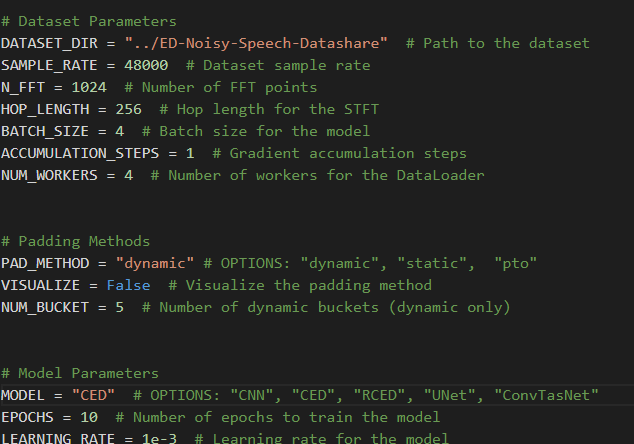
\includegraphics[width=0.8\textwidth]{dataset_config.png}
    \caption{\label{fig:dataset_config} Configuration of the CED model used for dataset performance evaluation.}
\end{figure}

Both uncached and cached runs were executed, and the relevant timing metrics were collected from the output logs, as shown in Table~\ref{tab:dataset_loading_times}.

\vspace{1em}
\begin{table}[H]
\centering
\caption{Training dataset preparation and runtime overheads (in seconds)}
\label{tab:dataset_loading_times}
\begin{tabular}{|l|c|c|c|}
\hline
\textbf{Dataset Type} & \textbf{Initial Load (Uncached)} & \textbf{Re-run Load (Cached)} & \textbf{Epoch Truncation Overhead (PTO only)} \\
\hline
Static Bucketing  & 298.05  & 0.81  & N/A    \\
Dynamic Bucketing & 602.56  & 0.58  & N/A    \\
PTO               & 311.21  & 0.58  & 58.56  \\
\hline
\end{tabular}
\end{table}

The results in Table~\ref{tab:dataset_loading_times} offer a clear overview of the dataset loading times and runtime overheads associated with each method. Static Bucketing proves to be the fastest in terms of initial load time, comprising only dataset loading and bucket assignment. Dynamic Bucketing incurs the highest overhead due to the computational cost of K-Means clustering. PTO, while slightly slower than Static Bucketing, remains efficient given that it must iterate through the dataset to compute the original waveform lengths.

The re-run loading times for all three methods are drastically reduced thanks to the use of cached data. All methods show comparable re-run times, with Static Bucketing being marginally slower.

A key distinction lies in the \textit{epoch truncation overheads}. Only the PTO method incurs this overhead due to its need to truncate outputs during training and evaluation to match the original input lengths. This step is unnecessary for the other two methods. While the added runtime is relatively minor in the context of total training time (typically in the order of hours), this overhead can scale significantly with larger datasets or more training epochs.

To evaluate the impact of dataset handling strategies on model learning, all models were compared using their best training checkpoint. Since the difference between cached and uncached runs was negligible in terms of performance, only the cached results are reported in Table~\ref{tab:dataset_performance}.

\vspace{1em}
\begin{table}[H]
\centering
\caption{Model Training Performance Across Dataset Handling Strategies}
\label{tab:dataset_performance}
\begin{tabular}{|l|c|c|c|}
\hline
\textbf{Dataset Type} & \textbf{Training Loss} & \textbf{Validation Loss} & \textbf{Validation SNR} \\
\hline
Static Bucketing  & 0.8367  & 0.8410  & 1.09 dB \\
Dynamic Bucketing & 0.8262  & 0.8298  & 1.10 dB \\  
PTO               & 0.6288  & 0.6633  & 1.10 dB \\
\hline
\end{tabular}
\end{table}

The results in Table~\ref{tab:dataset_performance} indicate that the model achieves comparable performance across all dataset handling methods. The consistent validation SNR values confirm that each method was implemented correctly and that the model learned similar representations regardless of the input formatting.

Interestingly, the PTO method shows a slightly lower training and validation loss. This discrepancy is not reflected in the SNR metric and may be attributed to differences in how output sequences are truncated during training. The closeness of training and validation losses across all configurations suggests that the model generalizes well and is neither underfitting nor overfitting.

\chapter{Future Work}
\label{chap:future_work}

While the project successfully met its primary goal of developing and evaluating a modular speech enhancement system. There remains considerable scope for future work. The pipeline was deliberately designed for modularity, allowing straightforward integration of emerging model architectures. Recent transformer based and diffusion based speech enhancement methods could be incorporated into the existing framework and evaluated using the same metrics. These models may offer gains in both perceptual and numerical performance.

For instance, the transformer based ScaleFormer model \cite{wu2023scaleformer}
is a very powerful architecture used in other domains. It was not implemented due to time constraints and the already high performance achieved, but its results indicate promising future potential. Effectively adapting such models to the spectrogram-based pipeline used here will be key to their success.

Another area for improvement is generalisation. As shown in Appendix~\ref{sec:pretrained_comparison}, both our best model and many pretrained systems struggled with unseen noise types. One outlier, \texttt{DeepFilterNet}, likely benefited from training on a more diverse dataset. This underscores the importance of exposing models to broader training data to ensure better real-world robustness. Since the pipeline was built from scratch. More advanced learning strategies such as reinforcement learning or self-supervised pretraining were not explored. These could accelerate convergence and improve generalisation, especially for larger models or more complex tasks.

Deployment-oriented enhancements also merit investigation. Real devices like headphones and smartphones often use microphone arrays, enabling spatial filtering. Future work could incorporate multichannel input and beamforming to better exploit these cues. Additionally, increased market interest and research into systems integrating playback time feedback or \gls{anc} has been seen. Its development does not reach too far from the current pipeline and evaluation could provide valuable insights.

Overall, the flexibility of the current system lays a strong foundation for continued experimentation and development. By extending its capabilities with newer architectures, more diverse data, and real-world constraints, the project can evolve into a deployable solution fit for modern audio enhancement demands.



\chapter{Conclusion}
\label{chp:conclusion}

This project set out to explore and compare classical and \gls{ml} approaches for speech enhancement. A modular pipeline was implemented, supporting flexible experimentation through custom dataset loaders, real-time inference support, and unified evaluation metrics. Critical implementation flaws, such as the improper use of \texttt{Tanh} activations, were identified and resolved through iterative metric-based and visual analysis.

Evaluation began with classical methods: \gls{ss}, \gls{wf}, and \gls{mmse-lsa}, establishing a reliable performance baseline. The project then introduced and assessed five \gls{ml} models—\gls{cnn}, \gls{ced}, \gls{rced}, \gls{unet}, and \gls{convtasnet}. All trained from scratch in the spectrogram domain using the Edinburgh DataShare dataset \cite{edinburghdataset}. A key contribution was the design and evaluation of variable-length dataset handling strategies, including static and dynamic bucketing and padding-truncation approaches. These ensured efficient training across sequences of diverse lengths.

To address hardware limits, \gls{oom} mitigation strategies were implemented. While these slightly reduced training accuracy, they consistently improved denoising metrics and enabled deeper models like \gls{unet} and \gls{convtasnet} to be trained successfully. \gls{convtasnet} emerged as the top performer, achieving an \gls{snr} of 18.06~dB, \gls{pesq} of 2.43, and \gls{stoi} of 0.91. Although training was computationally intensive, with ConvTasNet taking over 25 hours, these were one-time offline costs. Inference remained efficient, with the entire test set denoised in under two minutes. As summarised in Table~\ref{tab:summary_comparison}, this represents a substantial improvement over the best classical method, \gls{wf}, which achieved an \gls{snr} of 0.46~dB and \gls{pesq} of 2.06. The performance gap across all metrics highlights the clear advantage of data-driven \gls{ml} approaches in enhancing both numerical fidelity and perceptual quality, even when trained from scratch.

\vspace{1em}
\begin{table}[H]
\centering
\caption{Best Classical vs Best ML Denoising Performance}
\label{tab:summary_comparison}
\begin{tabular}{|l|c|c|c|c|c|}
\hline
\textbf{Model} & \textbf{↑SNR (dB)} & \textbf{↓MSE} & \textbf{↑PESQ} & \textbf{↑STOI} & \textbf{↓LSD (dB)} \\
\hline
\gls{wf} (Best Classical) & 0.46 & 0.002875 & 2.06 & 0.89 & 0.75 \\
\gls{convtasnet} (Best ML) & 18.06 & 0.000063 & 2.43 & 0.91 & 0.67 \\
\hline
\end{tabular}
\end{table}
\vspace{1em}

In conclusion, this project demonstrated the viability of training speech enhancement models from scratch using a well-engineered system. The final pipeline supports robust evaluation and real-time denoising, validating \gls{ml}-based approaches as a practical and superior alternative to classical methods. This work lays the foundation for potential future developments discussed in Chapter~\ref{chp:future_work}.


\printbibliography[title=References]

\appendix{}

\chapter{Project Structure}
\label{appendix:project_structure}

The overall structure of the project is modular, enabling clean separation of concerns and supporting future extensibility. The project is organised around two main pipelines \textbf{training} and \textbf{denoising}. Each pipeline is implemented as a collection of dedicated modules, coordinated through the central \texttt{main.py} script, which serves as the entry point for running the system.

To maintain clarity and modularity, all helper modules are organised within a \textit{Utils} directory. This directory contains the core functionality for dataset handling, \gls{ml} model definitions, training routines, inference logic, and classical baseline methods. Additionally, a centralised configuration file, \texttt{config.py}, located alongside \texttt{main.py}, manages all project parameters using a dictionary-based structure. This design allows users to easily modify hyperparameters or experiment settings in a single location, improving usability and reproducibility.

An overview of the key files in the \textit{Utils} directory is provided below:

\begin{itemize}
    \item \texttt{dataset.py}: Contains all dataset classes used in the project, implemented as PyTorch \texttt{Dataset} objects. The file supports multiple strategies for handling variable-length audio inputs, as discussed in Section~\ref{sec:datasets}. Along with the neccesary helper functions.

    \item \texttt{model.py}: Defines the \gls{ml} model architectures used for speech enhancement. Each model is implemented as a subclass of PyTorch’s \texttt{nn.Module}, and the module is designed for easy experimentation with new architectures or changes in hyperparameters. Many implementations had to be adapted from the original papers and the desing of such changes is discussed in Section~\ref{sec:model_architecture}.

    \item \texttt{train.py}: Implements the training loop, validation logic, and performance tracking. It supports training using any of the dataset classes defined in \texttt{dataset.py}. It also includes the \gls{oom} handeling disucssed in Section~\ref{sec:oom_handling} and justified in Section~\ref{sec:oom_validation}

    \item \texttt{denoise.py}: Handles inference and evaluation post-training. It defines two core functions: \texttt{batch\_denoise}, for full-dataset evaluation, and \texttt{single\_denoise}, for individual files. The module supports both \gls{ml}-based and classical methods, enabling seamless switching between approaches. It also includes \texttt{compute\_metrics}, which calculates objective metrics such as \gls{snr}, \gls{mse}, \gls{lsd}, \gls{pesq}, and \gls{stoi}, with all except \gls{lsd} computed using library functions. Metric calculations are consistent throughout the project. Classical methods, including \gls{ss}, \gls{wf}, and \gls{mmse-lsa}, are self-implemented to support spectrogram-based processing.

\end{itemize}

\graphicspath{{content/appendices/figures}}
\chapter{Suppression Effects from Improper \texttt{Tanh} Activation}
\label{appendix:tanh_removal}

Before final evaluations could be conducted, a critical implementation flaw affecting early model performance was identified. Initially all \gls{ml} models, except \gls{convtasnet}, included a \texttt{Tanh} activation function at the output layer. This was based on the assumption that constraining the real and imaginary spectrogram outputs to the range \([-1, 1]\) would improve numerical stability during \gls{istft} reconstruction.

However, during early testing and visualization, this constraint was found to significantly suppress amplitude dynamics. The outputs became unnaturally flattened, leading to degraded waveform clarity and poor denoising metrics. \gls{snr}, \gls{pesq}, and \gls{stoi} scores in particular, even when models appeared to converge during training.

This effect is illustrated clearly in Figures~\ref{fig:suppresed_waveform} and~\ref{fig:suppresed_spectrogram}, models when trained with \texttt{Tanh} applied. The waveforms exhibit a flattened energy profile, and the spectrograms lack contrast and high-frequency content.

\begin{figure}[H]
    \centering
    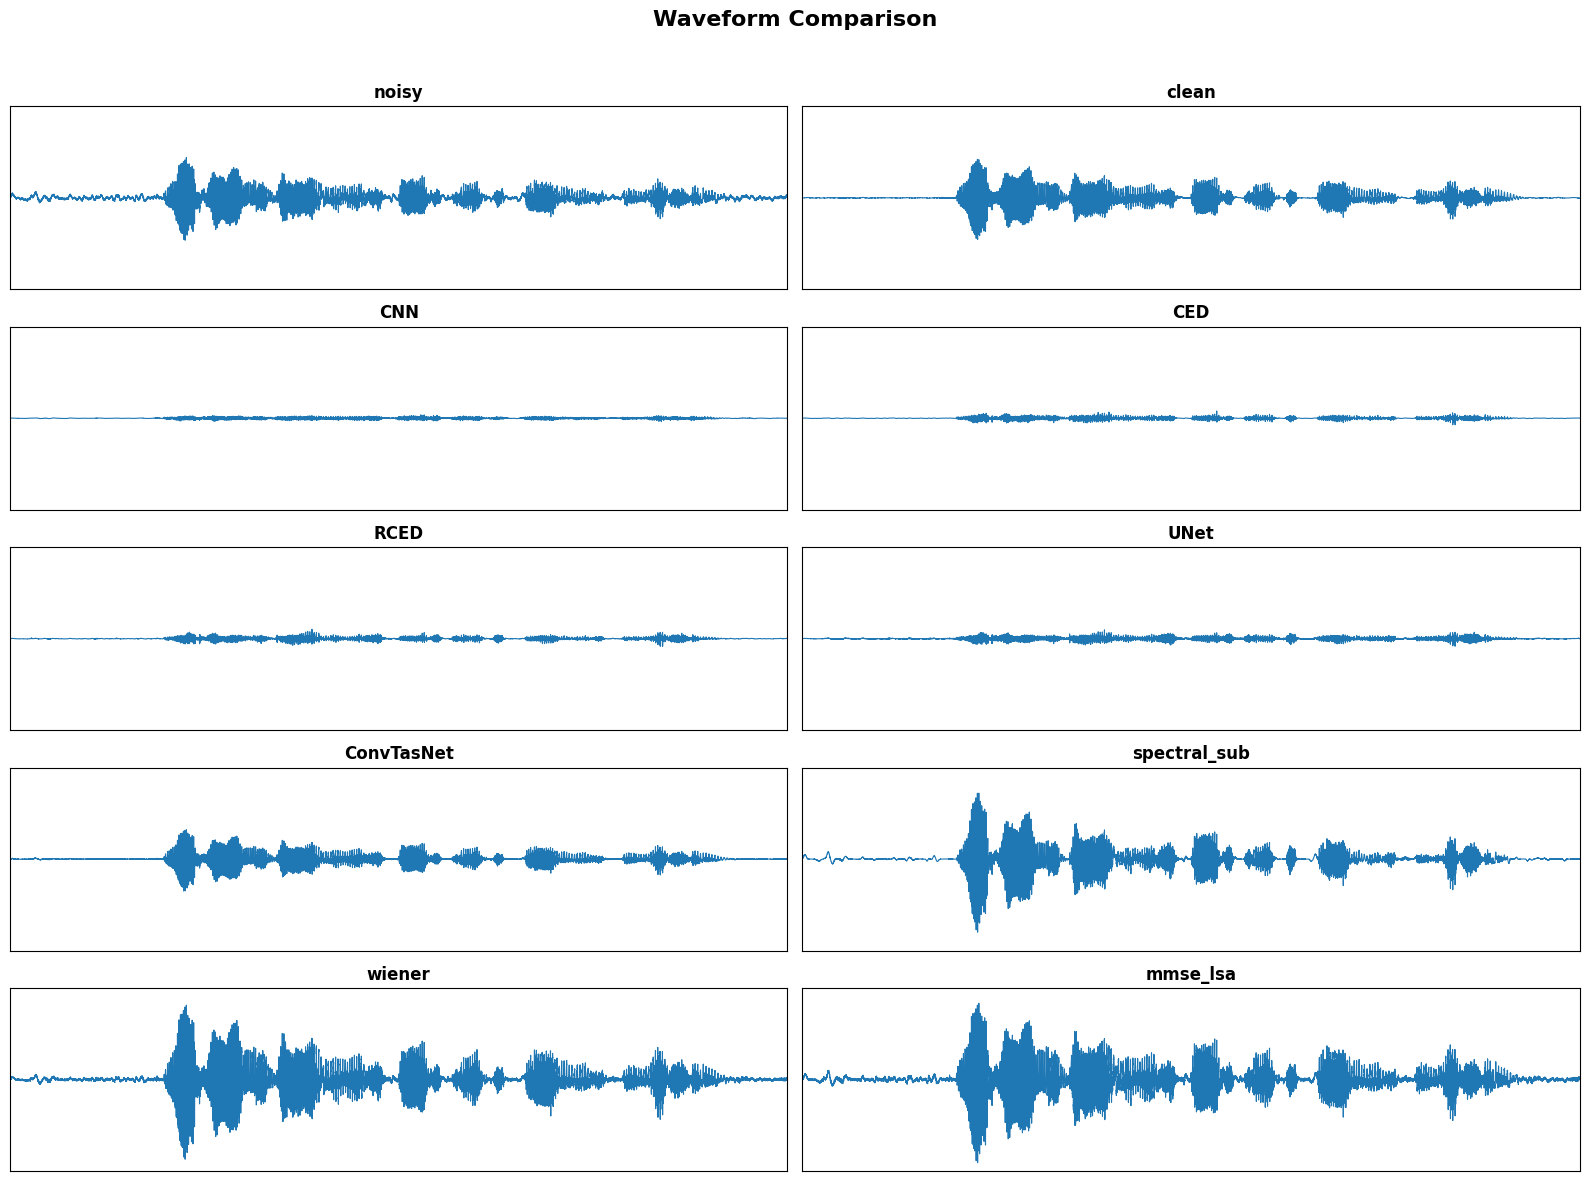
\includegraphics[width=0.9\textwidth]{suppresed_waveform.png}
    \caption{\label{fig:suppresed_waveform} Flattened waveform energy caused by \texttt{Tanh} activation. Output amplitude is artificially suppressed.}
\end{figure}

\begin{figure}[H]
    \centering
    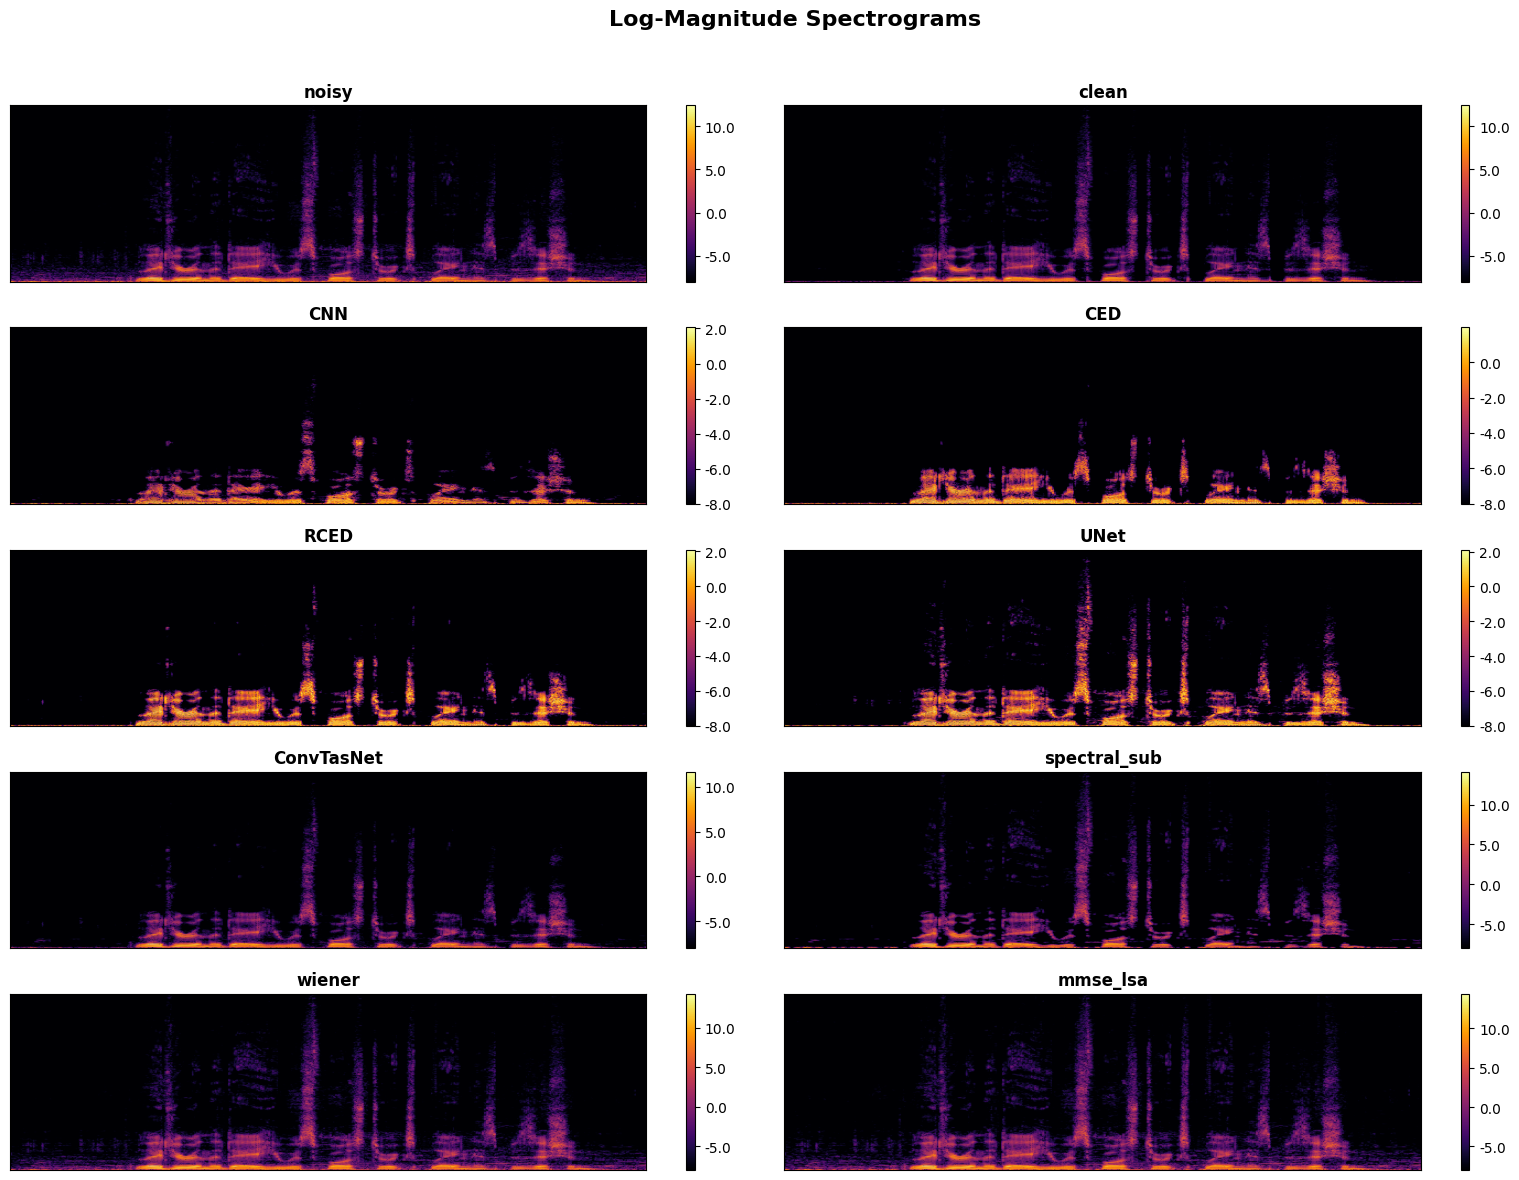
\includegraphics[width=0.9\textwidth]{suppresed_spectrogram.png}
    \caption{\label{fig:suppresed_spectrogram} Spectrograms with \texttt{Tanh} activation exhibit reduced contrast and dynamic range.}
\end{figure}

After removing \texttt{Tanh}, the models were retrained. The resulting outputs restored amplitude range and natural structure, both in waveform shape and spectrogram clarity. These improvements are shown in Figures~\ref{fig:restored_waveform} and~\ref{fig:restored_spectrogram}.

\begin{figure}[H]
    \centering
    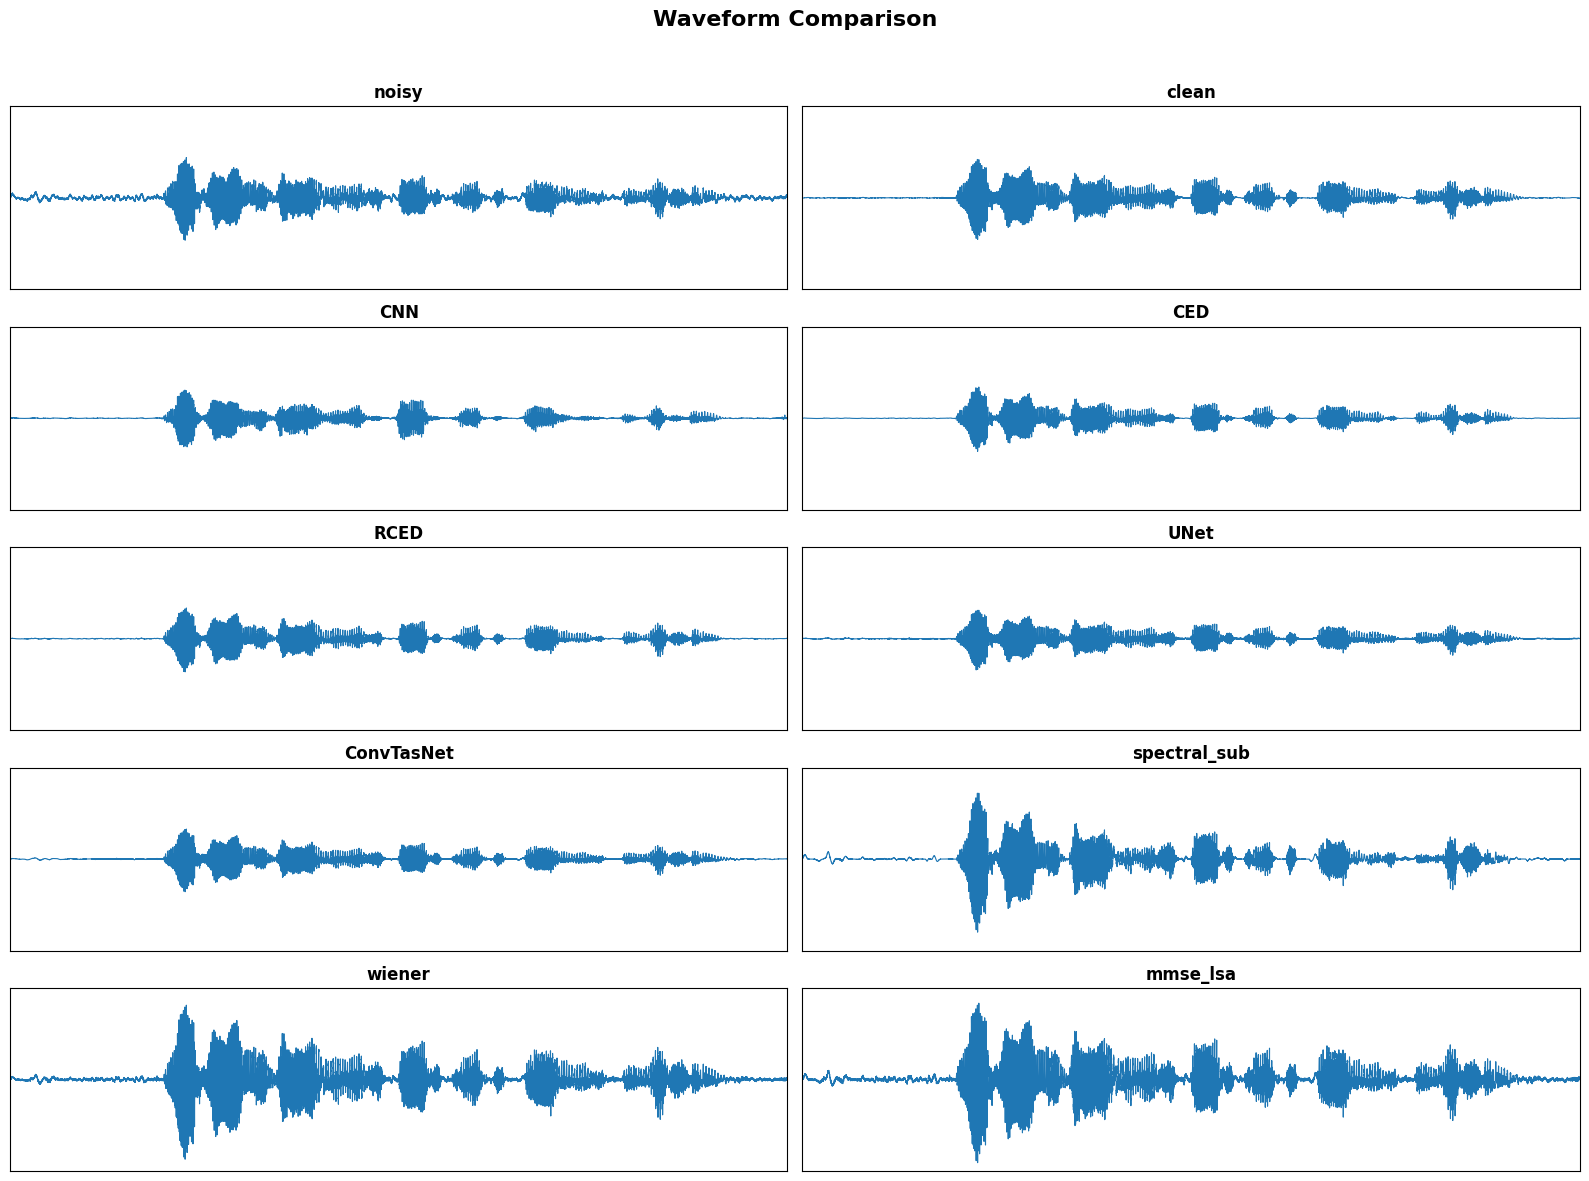
\includegraphics[width=0.9\textwidth]{fixed_waveform.png}
    \caption{\label{fig:restored_waveform} Corrected waveform comparison after removing \texttt{Tanh}. Energy and dynamics are restored.}
\end{figure}

\begin{figure}[H]
    \centering
    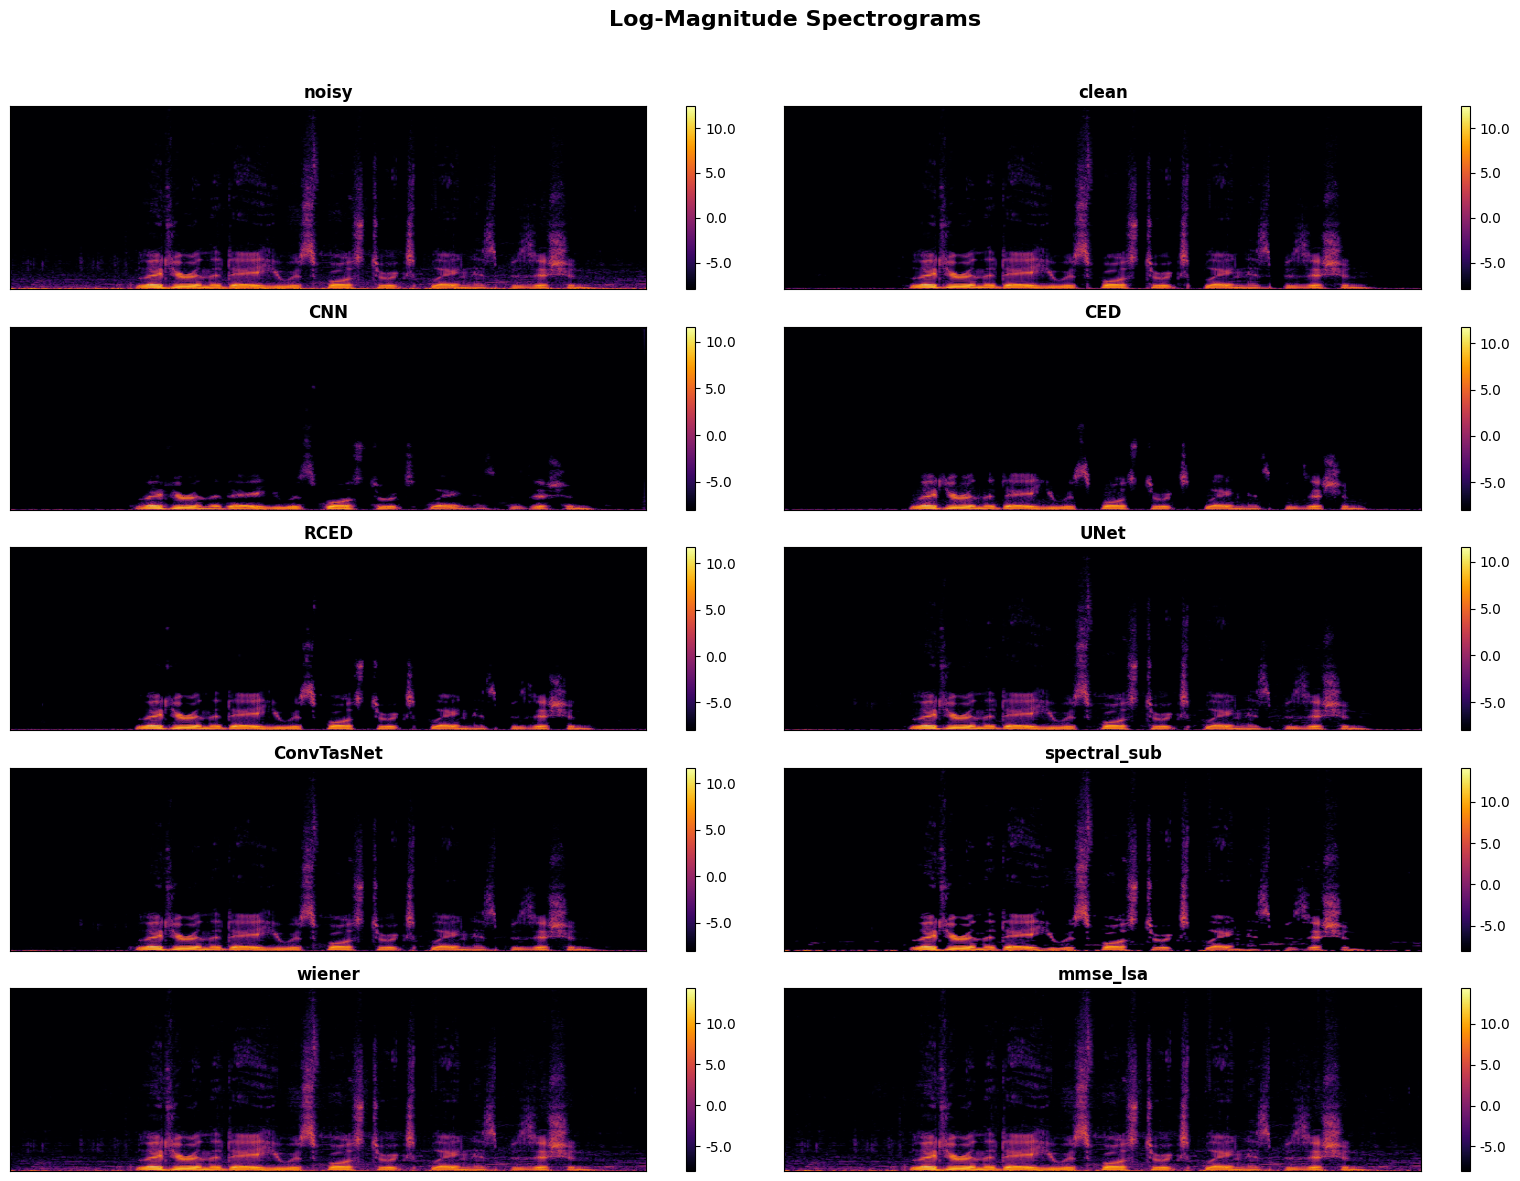
\includegraphics[width=0.9\textwidth]{fixed_spectrogram.png}
    \caption{\label{fig:restored_spectrogram} Log-magnitude spectrograms showing a restored dynamic range and greater clarity.}
\end{figure}

All final models, presented in Chapter~\ref{chp:evaluation} were retrained without the \texttt{Tanh} activation. This correction proved critical to achieving meaningful denoising results and validates the importance of properly scaled output layers in spectrogram-based models.

\graphicspath{{content/appendices/figures}}
\chapter{Appendix C}
\label{appendix:appendix_c}

\section{Extra Evaluation}
\label{sec:extra_evaluation}

\subsection{Subjective Evaluation}
\label{sec:subjective_evaluation}


\subsection{Comparison with Pretrained Models}
\label{sec:pretrained_comparison}

The results in Table~\ref{tab:ml_denoise} clearly show ConvTasNet as our highest-performing model. Importantly, all models in this project were trained entirely from scratch on our chosen dataset and adapted from literature to work with spectrogram-domain data. While this yielded strong results, it also means that these models are inherently specialized to the data they were trained on, and may not generalize well to unseen or real-world audio conditions.

This underscores the value of pre-trained models in the field of speech enhancement. Pre-trained systems like \textit{Demucs}, \textit{VoiceFixer}, and \textit{DeepFilterNet} are designed to work across a wider range of audio conditions, having been trained on large and diverse datasets. They leverage transfer learning to adapt to new tasks or domains, which can be particularly beneficial when the target dataset is limited in size or diversity. These models are often built on architectures that have been shown to be effective with adavaneced techniques.

To contextualize the performance of our best model ConvTasNet. We compared it against these pre-trained systems, which are also designed for speech enhancement tasks. We used the same evaluation metrics as in our previous experiments and to ensure a fair comparison two samples are used for this single denoising task. The first sample is drawn from our native dataset, while the second is taken from the NOIZEUS~\cite{hu2007subjective}, a foreign simple benchmark dataset for speech enhancement research. This allows us to evaluate the generalization capabilities of these models across different datasets.

\vspace{1em}
\begin{table}[H]
\centering
\caption{Evaluation of Pretrained Models vs ConvTasNet (per sample)}
\label{tab:pretrained_eval}
\begin{tabular}{|l|l|c|c|c|c|c|}
\hline
\textbf{Sample} & \textbf{Model} & \textbf{↑SNR} & \textbf{↓MSE} & \textbf{↓LSD} & \textbf{↑PESQ} & \textbf{↑STOI} \\
\hline
p232\_334 & ConvTasNet      & 12.40 & 0.0002 & 0.471 & 2.85 & 0.993 \\
p232\_334 & Demucs          & -2.95 & 0.0093 & 0.928 & 1.21 & 0.099 \\
p232\_334 & VoiceFix        & -2.26 & 0.0079 & 0.966 & 1.19 & 0.009 \\
p232\_334 & DeepFilterNet   & 21.62 & 0.0000 & 0.460 & 3.56 & 0.992 \\
\hline
sp07      & ConvTasNet      & -5.85 & 0.0059 & 1.614 & 1.04 & 0.230 \\
sp07      & Demucs          & -4.95 & 0.0048 & 1.378 & 1.04 & 0.243 \\
sp07      & VoiceFix        & -7.37 & 0.0084 & 1.565 & 1.04 & 0.193 \\
sp07      & DeepFilterNet   & 4.25  & 0.0006 & 1.012 & 1.34 & 0.848 \\
\hline
\end{tabular}
\end{table}


The results in Table~\ref{tab:pretrained_eval} offer important insights into the generalization capabilities of our trained from scratch ConvTasNet model compared to large scale pretrained models.

For the \texttt{p232\_334} sample from our native dataset, ConvTasNet performs exceptionally well, achieving strong scores across all metrics. An SNR of \textbf{12.40 dB}, PESQ of \textbf{2.85}, and a near perfect STOI of \textbf{0.993}. This confirms the model’s robustness when applied to data similar to its training distribution. Interestingly, DeepFilterNet significantly outperforms ConvTasNet in SNR (\textbf{21.62 dB}) and PESQ (\textbf{3.56}), suggesting that either a superior architecture or a more advanced training strategy may have been used to achieve such state of the art results. It is unclear, however, whether DeepFilterNet had prior exposure to this dataset or whether the sample is also foreign to its training distribution.

In contrast, Demucs and VoiceFixer underperform on this native sample, with negative SNR values and extremely low intelligibility scores (STOI < 0.1). This suggests a mismatch between their design assumptions and the characteristics of our spectrogram domain dataset, or possibly issues in the integration process used to adapt these models to our evaluation pipeline.

The results shift significantly for the \texttt{sp07} sample from the NOIZEUS dataset~\cite{hu2007subjective}. Here, ConvTasNet's performance deteriorates, yielding a negative SNR of \textbf{-5.85 dB} and a PESQ of \textbf{1.04}. This decline is expected given the differences in microphone quality, noise types, and recording environments. All of which present unseen conditions for our model. Similar trends are observed for Demucs and VoiceFixer, both of which also produce negative SNRs and generally lower perceptual scores. However, ConvTasNet still slightly outperforms them in perceptual metrics, suggesting a marginally better generalization capacity.

DeepFilterNet again shows the strongest generalization, maintaining a positive SNR of \textbf{4.25 dB} and a PESQ of \textbf{1.34}. While this performance is lower than its results on our native sample, it remains superior to all other models. Indicating more robust generalization to foreign audio. This also suggests that the \texttt{sp07} file may be a particularly challenging test case due to its distinct noise profile and recording setup.

Overall, these results validate both the strengths and limitations of our trained from scratch models. ConvTasNet performs strongly within its domain but struggles with generalization. Highlighting the challenge of deploying domain specific models in uncontrolled environments. Conversely, pretrained models particularly DeepFilterNet, demonstrate better cross-domain resilience. Underscoring the value of large scale, diverse training data and advanced model design when targeting real-world deployment.

\begin{figure}[H]
\centering
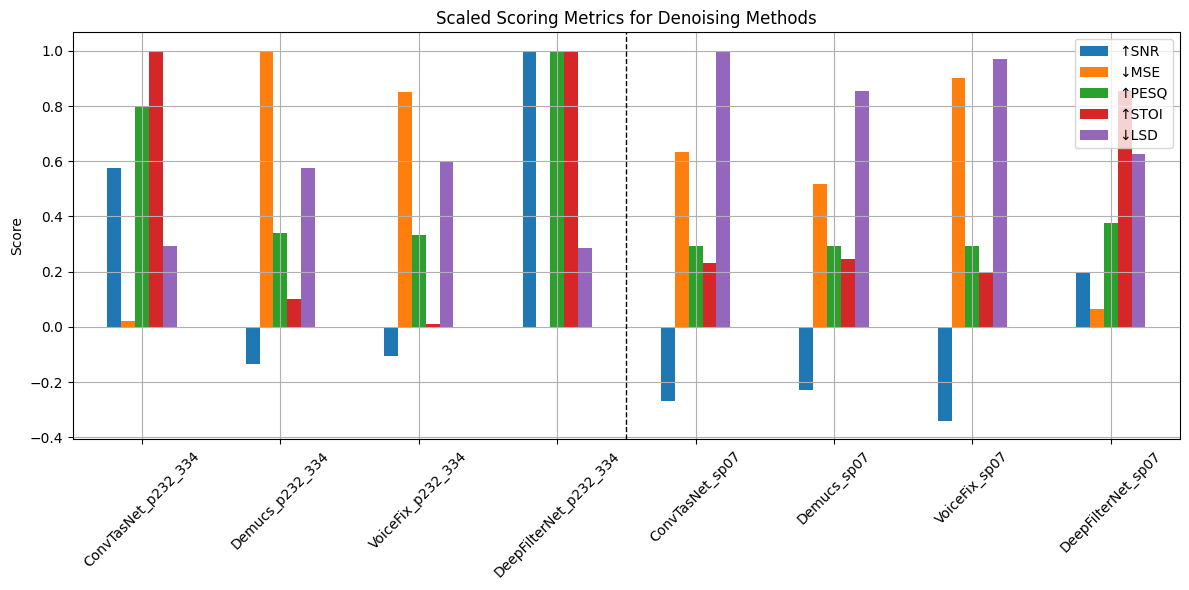
\includegraphics[width=1\textwidth]{pre_trained_metrics.png}
\caption{Scaled Scoring of ConvTasNet vs Pretrained Models}
\label{fig:pretrained_metrics}
\end{figure}
\noindent

Figure~\ref{fig:pretrained_metrics} provides a visual representation of the evaluation metrics for both ConvTasNet and the pretrained models. The scores are normalized to facilitate better visual comparison.



\end{document}
